\section{Cournot competition, entry, collusion and the concentration-margin relation}\label{sec:C-cournot}

Cross-industry studies in the structure-conduct-performance tradition relate profitability to
concentration. \citet{Bain1951} compared profit rates across industries, and later work regressed price-cost
margins on concentration \citep{Schmalensee1989}. This problem works out what four canonical models of a homogeneous-good
industry imply for that relation, and what the relation can and cannot say about mergers. The four models
are Cournot competition and perfect collusion, each with a fixed number of firms and with free entry. Two
extensions add firms with different costs and mergers. A computational part simulates a cross-section of
industries and compares the merger predictions of the regression with the true equilibrium effects. The
theory behind the problem is developed in \cref{sec:02-cournot,sec:02-entry,sec:02-collusion}, and the
cross-industry regression is studied in \cref{sec:01-montecarlo}.

\subsection{Statement}\label{sec:C-cournot-statement}

A homogeneous good has linear inverse demand $P(Q) = a - bQ$, where $Q$ is total output, $a > c > 0$ and
$b > 0$. Every active firm pays a fixed cost $F > 0$ per period and produces at constant marginal cost $c$. The
Lerner index is $L = \frac{P - c}{P}$, the Herfindahl index is $\HHI = \sum_i s_i^2$ with market shares
$s_i = \frac{q_i}{Q}$, and $\varepsilon = -\frac{\dd Q}{\dd P}\frac{P}{Q}$ is the market elasticity of demand,
written as a positive number. Two constants recur. The \emph{market-size index} is
$x \equiv \frac{a - c}{\sqrt{bF}}$, and the \emph{profit scale} is $k \equiv \frac{(a - c)^2}{b}$.

\begin{enumerate}[label=(\alph*)]
\item There are $N$ firms that choose outputs simultaneously. Describe the game and the equilibrium concept.
  Show that the equilibrium is unique and symmetric. Compute the price, outputs, profits, $L$ and $\HHI$, and
  verify that $L = \frac{\HHI}{\varepsilon}$.
\item Firms first decide whether to enter and then play the game of part (a). Treating the number of firms as
  continuous, find the free-entry number of firms and the resulting price, outputs, $L$ and $\HHI$.
\item Repeat parts (a) and (b) when the active firms collude perfectly, charging the monopoly price and
  splitting output equally. Show that collusion is not a Nash equilibrium of the one-shot game. Find the
  discount factor above which grim-trigger strategies sustain collusion in the infinitely repeated game.
\item Describe the relation between $\HHI$ and $L$ in the four cases.
\item An economist posits $\E[L] = \beta_0 + \beta_1\HHI$ and estimates it on a cross-section of industries.
  Does the specification make sense under each model? Are the estimates consistent, and for what? Are they
  useful for predicting the effect of a merger?
\item Let firm $i$ have its own constant marginal cost $c_i$, with every firm active. Show that
  $L_i = \frac{s_i}{\varepsilon}$ and $\sum_i s_iL_i = \frac{\HHI}{\varepsilon}$. Show that a mean-preserving spread
  of costs that keeps every firm active raises $\HHI$ and the share-weighted Lerner index, leaves the price
  unchanged and raises welfare.
\item Evaluate every object of parts (a) to (c) for $a = 10$, $c = 2$, $b = 1$ and $F = 1$, including consumer
  surplus, total welfare and the welfare-maximizing number of firms.
\item In the symmetric Cournot model, study the profitability of a merger of two firms and of $k_M$ firms.
  Compare the change in $\HHI$ computed from pre-merger shares with the equilibrium change. Find the marginal
  cost of the merged firm below which the merger does not raise the price.
\item (Computational.) Simulate a cross-section of Cournot industries, estimate the regression of part (e),
  and compare the merger effects it predicts with the true equilibrium effects.
\end{enumerate}

\subsection{Solution}\label{sec:C-cournot-solution}

\casehead{Part (a)}
The game has players $i = 1, \dots, N$. Each player chooses an output $q_i \ge 0$, all players move
simultaneously, and all primitives are common knowledge. Firm $i$'s payoff is
\begin{equation}\label{eq:C-cournot-profit}
\pi_i(q_i, q_{-i}) = \big(a - bQ - c\big)q_i - F, \qquad Q = q_i + Q_{-i}, \quad Q_{-i} = \sum_{j \ne i} q_j .
\end{equation}
A \emph{Nash equilibrium} is a profile $q^* = (q_1^*, \dots, q_N^*)$ such that $q_i^*$ maximizes
$\pi_i(q_i, q_{-i}^*)$ for every $i$. The fixed cost lowers the profit of an active firm but does not affect
its output choice.

Profit is strictly concave in the firm's own output, since
\begin{equation*}
\frac{\partial \pi_i}{\partial q_i} = a - c - bQ_{-i} - 2bq_i, \qquad
\frac{\partial^2 \pi_i}{\partial q_i^2} = -2b < 0 .
\end{equation*}
The unique best response to rivals' total output $Q_{-i}$ is therefore
\begin{equation}\label{eq:C-cournot-br}
BR_i(Q_{-i}) = \max\Big\{0, \frac{a - c - bQ_{-i}}{2b}\Big\}.
\end{equation}

\begin{proposition}[Linear Cournot equilibrium]\label{prop:C-cournot}
With $a > c$, the Cournot game has a unique Nash equilibrium. It is symmetric, every firm is active, and
\begin{equation}\label{eq:C-cournot-q}
q = \frac{a - c}{b(N + 1)}, \qquad Q = \frac{N(a - c)}{b(N + 1)}, \qquad P = \frac{a + Nc}{N + 1}.
\end{equation}
\end{proposition}

\begin{proof}
We proceed in three steps. First, total output is positive in any equilibrium. If $Q = 0$, every firm faces
$Q_{-i} = 0$, and \eqref{eq:C-cournot-br} gives $BR_i(0) = \frac{a - c}{2b} > 0$, a contradiction. Second,
every firm is active. An active firm $l$ satisfies the first-order condition $a - c - bQ - bq_l = 0$, so
\begin{equation*}
bq_l = a - c - bQ .
\end{equation*}
Since $q_l > 0$, this gives $a - c - bQ > 0$. A firm $i$ with $q_i = 0$ would need
$\frac{\partial \pi_i}{\partial q_i}\big|_{q_i = 0} = a - c - bQ \le 0$, which contradicts the previous
inequality. Third, every firm satisfies $bq_i = a - c - bQ$, so all outputs are equal. Summing over the $N$
firms gives
\begin{align*}
bQ &= N(a - c) - NbQ, \\
Q &= \frac{N(a - c)}{b(N + 1)} .
\end{align*}
Total output is unique, so each output $q = \frac{Q}{N}$ is unique. The price is
$P = a - bQ = \frac{a(N + 1) - N(a - c)}{N + 1} = \frac{a + Nc}{N + 1}$.
\end{proof}

The remaining objects follow by substitution. The margin and the profit are
\begin{align}
P - c &= \frac{a + Nc - (N + 1)c}{N + 1} = \frac{a - c}{N + 1} = bq, \label{eq:C-cournot-margin}\\
\pi &= (P - c)q - F = \frac{a - c}{N + 1}\cdot\frac{a - c}{b(N + 1)} - F = \frac{k}{(N + 1)^2} - F .
\label{eq:C-cournot-pi}
\end{align}
The Lerner index divides the margin by the price, and every firm has share $\frac{1}{N}$:
\begin{equation}\label{eq:C-cournot-LH}
L = \frac{a - c}{N + 1}\cdot\frac{N + 1}{a + Nc} = \frac{a - c}{a + Nc}, \qquad
\HHI = N\cdot\frac{1}{N^2} = \frac{1}{N}.
\end{equation}
With linear demand $-\frac{\dd Q}{\dd P} = \frac{1}{b}$, so the elasticity at the equilibrium is
\begin{equation*}
\varepsilon = \frac{P}{bQ} = \frac{a + Nc}{N + 1}\cdot\frac{N + 1}{N(a - c)} = \frac{a + Nc}{N(a - c)} .
\end{equation*}
The check is direct:
$\frac{\HHI}{\varepsilon} = \frac{1}{N}\cdot\frac{N(a - c)}{a + Nc} = \frac{a - c}{a + Nc} = L$. The relation
holds for any demand curve. Firm $i$'s first-order condition $P + q_iP'(Q) = c$ gives
$\frac{P - c}{P} = -\frac{q_iP'}{P} = \frac{q_i}{Q}\cdot\frac{1}{\varepsilon}$, and symmetry sets
$\frac{q_i}{Q} = \frac{1}{N} = \HHI$ (\cref{sec:02-cournot-markups}).

\casehead{Part (b)}
Entry adds a first stage. In stage 1, a large pool of identical potential entrants decide simultaneously
whether to enter and pay $F$. In stage 2, the $N$ entrants observe $N$ and play the Cournot game of part (a).
The solution concept is \emph{subgame-perfect equilibrium}. \Cref{prop:C-cournot} fixes play in every
stage-2 subgame, so an entrant earns $\pi(N) = \frac{k}{(N + 1)^2} - F$, which is strictly decreasing in $N$.
In equilibrium no entrant regrets entering and no outsider wants to enter, so the number of firms $N^e$
satisfies $\pi(N^e) \ge 0 \ge \pi(N^e + 1)$. Treating $N$ as continuous gives the zero-profit condition
$\pi(N^e) = 0$:
\begin{align}
(N^e + 1)^2 &= \frac{(a - c)^2}{bF} = x^2, \notag\\
N^e &= x - 1 = \frac{a - c}{\sqrt{bF}} - 1 . \label{eq:C-Ne}
\end{align}
The free-entry outcomes follow from \eqref{eq:C-cournot-q} and \eqref{eq:C-cournot-margin} with
$\frac{a - c}{N^e + 1} = \sqrt{bF}$:
\begin{align}
P^e &= c + \frac{a - c}{N^e + 1} = c + \sqrt{bF}, \qquad
q^e = \frac{a - c}{b(N^e + 1)} = \frac{\sqrt{bF}}{b} = \sqrt{\frac{F}{b}}, \notag\\
Q^e &= \frac{a - P^e}{b} = \frac{a - c - \sqrt{bF}}{b}, \notag\\
L^e &= \frac{P^e - c}{P^e} = \frac{\sqrt{bF}}{c + \sqrt{bF}}, \qquad
\HHI^e = \frac{1}{N^e} = \frac{1}{x - 1} = \frac{\sqrt{bF}}{a - c - \sqrt{bF}} . \label{eq:C-free-entry}
\end{align}
Each entrant earns $(P^e - c)q^e - F = \sqrt{bF}\sqrt{\frac{F}{b}} - F = 0$. The formulas require $N^e \ge 1$,
that is, $x \ge 2$, or equivalently $0 < F \le \frac{(a - c)^2}{4b}$. The Cournot rule survives entry. The elasticity at
$P^e$ is $\varepsilon^e = \frac{P^e}{bQ^e} = \frac{c + \sqrt{bF}}{a - c - \sqrt{bF}}$, and
$\frac{\HHI^e}{\varepsilon^e} = L^e$. Under free entry the dollar margin $\sqrt{bF}$ is fixed by technology
and the slope of demand. A larger intercept $a$ brings more firms and leaves the margin unchanged. With the
integer constraint, $N^e$ is the integer part of $x - 1$ (\cref{sec:02-mw-integer}).

\casehead{Part (c)}
Under perfect collusion with $N$ firms fixed, the firms choose total output to maximize joint profit
\begin{equation*}
\Pi(Q) = (a - bQ - c)Q - NF, \qquad \Pi''(Q) = -2b < 0 .
\end{equation*}
The first-order condition $a - c - 2bQ = 0$ gives the monopoly outcome
\begin{equation}\label{eq:C-monopoly}
Q^m = \frac{a - c}{2b}, \qquad P^m = a - bQ^m = \frac{a + c}{2}, \qquad P^m - c = \frac{a - c}{2}.
\end{equation}
Each firm produces $q = \frac{Q^m}{N} = \frac{a - c}{2bN}$ and earns $\pi = \frac{a - c}{2}\cdot\frac{a - c}{2bN} - F
= \frac{k}{4N} - F$. The Lerner index is $L = \frac{a - c}{a + c}$ for every $N$, and $\HHI = \frac{1}{N}$. The
elasticity at the monopoly price is $\varepsilon(P^m) = \frac{P^m}{bQ^m} = \frac{a + c}{a - c}$, so
$L = \frac{1}{\varepsilon(P^m)}$, the monopoly inverse-elasticity rule. Price, total output and the margin do not
depend on $N$. Profit per firm and $\HHI$ fall as $N$ rises.

Collusion is not a Nash equilibrium of the one-shot game when $N \ge 2$. Suppose every rival produces
$\frac{Q^m}{N}$. At $q_i = \frac{Q^m}{N}$ the marginal profit of firm $i$ is
\begin{equation*}
\frac{\partial \pi_i}{\partial q_i} = a - c - bQ^m - b\frac{Q^m}{N} = \frac{a - c}{2} - \frac{a - c}{2N}
= \frac{(N - 1)(a - c)}{2N} > 0 .
\end{equation*}
Each firm gains by expanding, because it bears only its own share of the price reduction that its extra
output causes.

Collusion can be sustained in the infinitely repeated game. In periods $t = 0, 1, 2, \dots$ the $N$ firms play
the stage game of part (a). Outputs are observed at the end of each period. In this problem $\delta \in (0, 1)$
denotes the discount factor, as in \cref{ch:collusion-theory} (in the demand chapters $\delta$ is mean utility).
Firm $i$ maximizes $\sum_{t \ge 0}\delta^t\pi_{it}$. Under \emph{grim-trigger} strategies \citep{Friedman1971}, each
firm produces $\frac{Q^m}{N}$ in period 0 and in every period that follows no deviation. After any deviation every
firm produces the Cournot output $\frac{a - c}{b(N + 1)}$ forever.

\begin{proposition}[Threshold discount factor for Cournot collusion]\label{prop:C-delta}
Grim-trigger strategies form a subgame-perfect equilibrium that sustains the monopoly outcome if and only if
\begin{equation}\label{eq:C-delta}
\delta \ge \delta^*(N) \equiv \frac{(N + 1)^2}{N^2 + 6N + 1}.
\end{equation}
The threshold satisfies $\delta^*(2) = \frac{9}{17}$, is strictly increasing in $N$ for $N > 1$, and
tends to one as $N \to \infty$.
\end{proposition}

\begin{proof}
The fixed cost enters every period's payoff equally, so it cancels from every incentive constraint. What remains is
\cref{prop:12-cournot}, which gives the threshold, its monotonicity and its limit. At $N = 2$ the threshold is
$\frac{9}{4 + 12 + 1} = \frac{9}{17}$.
\end{proof}

\Cref{fig:C-delta} plots the threshold together with the Bertrand benchmark. In the Bertrand supergame a
deviator undercuts slightly and takes the whole monopoly profit $\pi^m$, after which profits are zero. The
condition $\frac{\pi^m}{N(1 - \delta)} \ge \pi^m$ gives $\delta \ge 1 - \frac{1}{N}$ (\cref{prop:12-bertrand}).
\citet[Section~6.3.2.1]{Tirole1988} uses this threshold to formalize the old claim that concentration facilitates
tacit collusion.
The two thresholds cross between $N = 2$ and $N = 3$. Cournot collusion is harder to sustain for $N = 2$
($\frac{9}{17} = 0.529$ against $0.5$) and easier for every $N \ge 3$ ($\frac{4}{7} = 0.571$ against $0.667$ at
$N = 3$). For large $N$, $1 - \delta^*(N) = \frac{4N}{N^2 + 6N + 1}$ is close to $\frac{4}{N}$, four
times the Bertrand slack $\frac{1}{N}$. Cournot reversion is a mild punishment, but the one-shot gain from
deviating is also small, because the deviator expands only to its best response.

\begin{figure}[htbp]
\centering
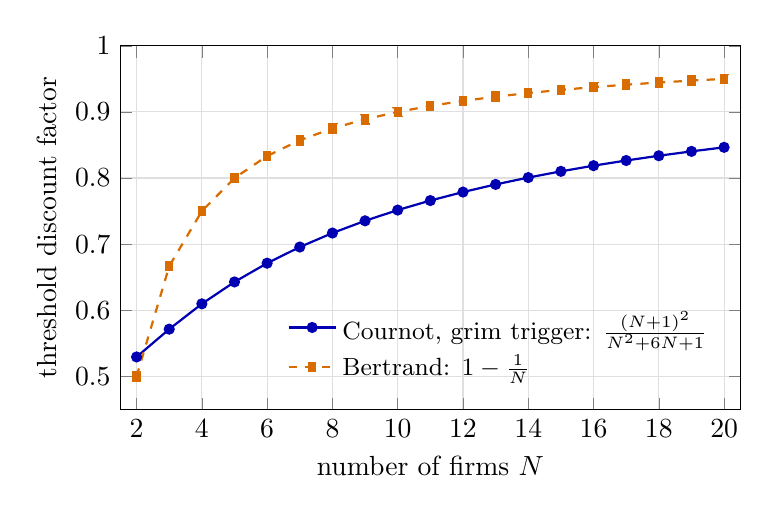
\begin{tikzpicture}
\begin{axis}[
  width=0.78\textwidth, height=6.2cm,
  xlabel={number of firms $N$}, ylabel={threshold discount factor},
  xmin=1.5, xmax=20.5, ymin=0.45, ymax=1.0,
  xtick={2,4,6,8,10,12,14,16,18,20},
  ytick={0.5,0.6,0.7,0.8,0.9,1.0},
  yticklabel style={/pgf/number format/fixed, /pgf/number format/precision=1},
  grid=major, grid style={gray!25},
  legend style={draw=none, fill=none, font=\small, at={(0.97,0.05)}, anchor=south east},
  legend cell align=left,
]
\addplot[blue!70!black, thick, mark=*, mark size=1.6pt, samples at={2,3,...,20}]
  {(x + 1)^2/(x^2 + 6*x + 1)};
\addlegendentry{Cournot, grim trigger: $\frac{(N + 1)^2}{N^2 + 6N + 1}$}
\addplot[orange!85!black, thick, dashed, mark=square*, mark size=1.5pt, samples at={2,3,...,20}]
  {1 - 1/x};
\addlegendentry{Bertrand: $1 - \frac{1}{N}$}
\end{axis}
\end{tikzpicture}
\caption{Lowest discount factor at which grim-trigger strategies sustain the monopoly outcome among $N$
symmetric firms, for Cournot and Bertrand stage games with linear demand and constant marginal cost. The
Cournot threshold does not depend on $a$, $b$, $c$ or $F$.}
\label{fig:C-delta}
\end{figure}

\begin{remark}
Grim trigger is not the harshest credible punishment. \citet{Abreu1986} studies stick-and-carrot
punishments, in which firms produce more than the Cournot output for one period and then return to
collusion. These punish deviators more severely and sustain the monopoly outcome at lower discount factors
than \eqref{eq:C-delta}. \Cref{ch:collusion-theory} develops optimal punishments.
\end{remark}

With free entry, collusive play in stage 2 yields per-firm profit $\pi(N) = \frac{k}{4N} - F$. The free-entry
condition $\pi(N^m) = 0$, with $N$ continuous, gives
\begin{equation}\label{eq:C-Nm}
N^m = \frac{(a - c)^2}{4bF} = \frac{x^2}{4}.
\end{equation}
Price and total output stay at the monopoly values, so entry only changes how $Q^m$ is divided:
\begin{equation*}
q^m = \frac{Q^m}{N^m} = \frac{a - c}{2b}\cdot\frac{4bF}{(a - c)^2} = \frac{2F}{a - c}, \qquad
L = \frac{a - c}{a + c}, \qquad \HHI^m = \frac{1}{N^m} = \frac{4bF}{(a - c)^2}.
\end{equation*}
Total fixed costs equal the monopoly profit, $N^mF = \frac{(a - c)^2}{4b} = (P^m - c)Q^m$, so entry dissipates
the whole rent. Consumers gain nothing, because the price stays at $P^m$. Collusion attracts more entrants
than Cournot competition:
\begin{equation}\label{eq:C-Nm-Ne}
N^m - N^e = \frac{x^2}{4} - x + 1 = \Big(\frac{x}{2} - 1\Big)^2 \ge 0,
\end{equation}
with equality only at $x = 2$, where both equal one. The higher collusive margin draws firms in until profit is
again zero. The collusive outcome with $N^m$ firms is an equilibrium of the repeated game only if $\delta \ge
\delta^*(N^m)$. Lower fixed costs raise $N^m$ and push the threshold toward one, so free entry also
makes collusion harder to enforce.

\casehead{Part (d)}
\Cref{tab:C-cournot-cases} collects the four regimes (the closed forms are also in
\cref{tab:02-linear-cournot}). Under Cournot conduct with $N$ fixed, substitute $N = \frac{1}{\HHI}$ in
the elasticity of part (a):
\begin{equation}\label{eq:C-LH-curve}
\varepsilon = \frac{a\HHI + c}{a - c}, \qquad L = \frac{\HHI}{\varepsilon} = \frac{(a - c)\HHI}{a\HHI + c}.
\end{equation}
The derivatives
\begin{align*}
\frac{\dd L}{\dd\HHI} &= \frac{(a - c)(a\HHI + c) - (a - c)\HHI a}{(a\HHI + c)^2} = \frac{c(a - c)}{(a\HHI + c)^2} > 0,\\
\frac{\dd^2 L}{\dd\HHI^2} &= -\frac{2ac(a - c)}{(a\HHI + c)^3} < 0
\end{align*}
show an increasing and concave curve. It runs from $L = 0$ at $\HHI = 0$ to the monopoly value
$\frac{a - c}{a + c}$ at $\HHI = 1$. When $N$ is set outside the model, the curve is the causal effect of
concentration on margins in an industry with given $(a, c)$.

\begin{table}[htbp]
\centering
\begin{threeparttable}
\caption{Concentration and margins in the linear homogeneous-good industry under four regimes}
\label{tab:C-cournot-cases}
\small
\setlength{\tabcolsep}{4pt}
\begin{tabular}{@{}lccccc>{\raggedright\arraybackslash}p{2.75cm}@{}}
\toprule
Regime & $N$ & $P$ & $q$ & $L$ & $\HHI$ & Relation of $L$ to $\HHI$ \\
\midrule
Cournot, fixed $N$ & $N$ & $\frac{a + Nc}{N + 1}$ & $\frac{a - c}{b(N + 1)}$ & $\frac{a - c}{a + Nc}$ &
  $\frac{1}{N}$ & increasing, concave, causal \\
\addlinespace
Cournot, free entry & $x - 1$ & $c + \sqrt{bF}$ & $\sqrt{\frac{F}{b}}$ & $\frac{\sqrt{bF}}{c + \sqrt{bF}}$ &
  $\frac{\sqrt{bF}}{a - c - \sqrt{bF}}$ & same curve, both endogenous \\
\addlinespace
Collusion, fixed $N$ & $N$ & $\frac{a + c}{2}$ & $\frac{a - c}{2bN}$ & $\frac{a - c}{a + c}$ & $\frac{1}{N}$ &
  flat \\
\addlinespace
Collusion, free entry & $\frac{x^2}{4}$ & $\frac{a + c}{2}$ & $\frac{2F}{a - c}$ & $\frac{a - c}{a + c}$ &
  $\frac{4bF}{(a - c)^2}$ & opposite directions when $a$ or $c$ vary \\
\bottomrule
\end{tabular}
\begin{tablenotes}\footnotesize
\item Notes: Inverse demand $P = a - bQ$, marginal cost $c$, fixed cost $F$, and $x = \frac{a - c}{\sqrt{bF}}$.
Free-entry columns treat $N$ as continuous and require $x \ge 2$. Under Cournot conduct $L = \frac{\HHI}{\varepsilon}$,
and under collusion $L = \frac{1}{\varepsilon}$, with $\varepsilon$ evaluated at the equilibrium price.
\end{tablenotes}
\end{threeparttable}
\end{table}

With free entry, Cournot industries stay on the curve \eqref{eq:C-LH-curve}, but $\HHI^e$ and $L^e$ are now
both outcomes of $(a, b, c, F)$. Write $r = \sqrt{bF}$, so that $\HHI^e = \frac{r}{a - c - r}$ and
$L^e = \frac{r}{c + r}$. Each primitive moves the pair differently. A higher $F$ or $b$ raises $r$ and with it
both $\HHI^e$ and $L^e$, so the industry moves up along the curve. A higher $a$ lowers $\HHI^e$ and leaves $L^e$
unchanged. A higher $c$ raises $\HHI^e$ and lowers $L^e$. Across industries, the sign of the association
between $\HHI$ and $L$ therefore depends on which primitive varies.

Under collusion with $N$ fixed, $L = \frac{a - c}{a + c}$ for every $N$, so the relation is flat. With free
entry, $L$ still depends only on $(a, c)$, while $\HHI^m = \frac{4bF}{(a - c)^2}$. Variation in $F$ or $b$
moves $\HHI^m$ alone. A higher $a$ raises $L$ and lowers $\HHI^m$, and a higher $c$ does the reverse, so
variation in $a$ or $c$ moves the two indices in opposite directions.

Differences in conduct weaken, and can reverse, the positive Cournot relation. Compare a Cournot industry and
a collusive industry with the same primitives. With $N$ fixed both have $\HHI = \frac{1}{N}$, and the collusive
industry has the higher margin, since $\frac{a - c}{a + c} > \frac{a - c}{a + Nc}$ for $N > 1$. With free entry,
collusion again raises the margin, because $P^e = c + \sqrt{bF} \le \frac{a + c}{2} = P^m$ whenever $x \ge 2$.
By \eqref{eq:C-Nm-Ne} the collusive industry is also less concentrated. A cross-section that mixes the two
pairs high margins with low concentration. This pulls the slope of $L$ on $\HHI$ below the Cournot curve and
can make it negative. \Cref{fig:02-LH} draws the four cases for $a = 10$ and $c = 2$.

\casehead{Part (e)}
The specification $\E[L] = \beta_0 + \beta_1\HHI$ fits the four models to different degrees.
\begin{itemize}
\item Cournot, fixed $N$. The model implies $L = \frac{\HHI}{\varepsilon}$, so $\beta_0 = 0$ and margins rise
  with $\HHI$. The relation is linear with $\beta_1 = \frac{1}{\varepsilon}$ only if $\varepsilon$ is the same in
  every industry. With linear demand, $\varepsilon = \frac{a\HHI + c}{a - c}$ rises with $\HHI$ by
  \eqref{eq:C-LH-curve}, so the true relation is concave and the linear form is an approximation.
\item Cournot, free entry. Industries still lie on $L = \frac{\HHI}{\varepsilon}$, so the specification remains
  an approximation. Differences in $\HHI$ now reflect differences in $(a, b, c, F)$.
\item Collusion, fixed $N$. The margin does not depend on $\HHI$, so the specification holds only in the
  degenerate form $\beta_1 = 0$.
\item Collusion, free entry. A nonzero slope can arise from joint variation of the primitives, and it has no
  causal meaning.
\end{itemize}

Cross-industry OLS converges to $\frac{\Cov(L, \HHI)}{\Var(\HHI)}$ (\cref{prop:01-scp-plim}). This limit
summarizes the joint distribution of outcomes. It equals a structural parameter such as $\frac{1}{\varepsilon}$
only under special conditions, and four problems separate the two. First, concentration is endogenous, because the same primitives determine
$\HHI$ and $L$, and part (d) shows that even the sign of the association depends on which primitive varies.
Second, industries differ in elasticity and conduct, so $\hat\beta_1$ averages over different models. If
$L_k = \frac{\HHI_k}{\varepsilon_k}$ with $\varepsilon_k$ independent of $\HHI_k$, the slope converges to
$\E[\frac{1}{\varepsilon_k}]$, and otherwise it does not. Third, accounting margins differ from economic
margins. Measured price-cost margins omit the cost of capital, and capital intensity is correlated with
fixed costs and hence with $\HHI$. Fourth, $\HHI$ is measured with error and depends on the market definition,
which attenuates the slope.

Even a positive and precisely estimated $\hat\beta_1$ need not mean that concentration raises margins.
Part (f) shows that when firms differ in costs, efficient firms are large, so concentration and the average
margin rise together while welfare also rises. This is the efficiency critique of \citet{Demsetz1973}.

The regression is a weak tool for merger prediction. The economist would compute
$\widehat{\Delta L} = \hat\beta_1\,\Delta\HHI$ with $\Delta\HHI = 2s_is_j$ from the merging firms' pre-merger
shares. The prediction inherits every bias of $\hat\beta_1$. The share-based $\Delta\HHI$ also misstates the
equilibrium change in concentration (part (h)), and the prediction ignores entry, coordinated effects and
cost savings. Part (i) measures the size of these errors in simulated data.

\casehead{Part (f)}
Let firm $i$ have constant marginal cost $c_i$ and suppose all $N$ firms are active. The first-order
condition of firm $i$ is $a - bQ - bq_i - c_i = 0$, that is,
\begin{equation}\label{eq:C-asym-foc}
bq_i = P - c_i .
\end{equation}
Summing over firms gives $bQ = Na - \sum_j c_j - NbQ$, so
\begin{equation}\label{eq:C-asym}
Q = \frac{Na - \sum_j c_j}{b(N + 1)}, \qquad P = a - bQ = \frac{a + \sum_j c_j}{N + 1}, \qquad
q_i = \frac{a + \sum_j c_j - (N + 1)c_i}{b(N + 1)} .
\end{equation}
All firms are active if and only if $c_i < P$ for every $i$. Dividing \eqref{eq:C-asym-foc} by $P$,
\begin{equation*}
L_i = \frac{P - c_i}{P} = \frac{bq_i}{P} = \frac{q_i}{Q}\cdot\frac{bQ}{P} = \frac{s_i}{\varepsilon},
\qquad
\sum_i s_iL_i = \frac{1}{\varepsilon}\sum_i s_i^2 = \frac{\HHI}{\varepsilon} .
\end{equation*}
The share-weighted Lerner index equals the Herfindahl index divided by the market elasticity
\citep{CowlingWaterson1976}. The same steps apply to any demand curve, because the first-order condition
$P + q_iP' = c_i$ gives $L_i = \frac{s_i}{\varepsilon}$ directly. The ratio of industry variable profit to revenue is
the same object,
\begin{equation*}
\frac{\sum_i(P - c_i)q_i}{PQ} = \sum_i\frac{q_i}{Q}\cdot\frac{P - c_i}{P} = \sum_is_iL_i = \frac{\HHI}{\varepsilon} ,
\end{equation*}
which is Exercise~5.6 of \citet[Section~5.5]{Tirole1988}.

A \emph{mean-preserving spread} of costs is a change from $(c_i)$ to $(c_i')$ with
$\sum_i c_i' = \sum_i c_i$ and $\sum_i(c_i' - \bar c)^2 > \sum_i(c_i - \bar c)^2$, where $\bar c$ is the mean cost.
We write $\Var(c) = \frac{1}{N}\sum_i(c_i - \bar c)^2$ for the cross-firm variance.

\begin{proposition}[Cost dispersion, concentration and welfare]\label{prop:C-demsetz}
In the linear Cournot model with all firms active, a mean-preserving spread of marginal costs that keeps
every firm active leaves $Q$, $P$, $\varepsilon$ and consumer surplus unchanged. It raises $\HHI$ and the
share-weighted Lerner index, and it raises total welfare by $\frac{N\Delta\Var(c)}{b}$, where $\Delta\Var(c)$
is the increase in the cost variance.
\end{proposition}

\begin{proof}
We use four steps. First, by \eqref{eq:C-asym} total output and the price depend on costs only through
$\sum_j c_j$, which the spread holds fixed. Hence $Q$, $P$, the elasticity $\varepsilon = \frac{P}{bQ}$ and
consumer surplus $\frac{bQ^2}{2}$ are unchanged. Second, by \eqref{eq:C-asym-foc} outputs are
$q_i = \frac{P - c_i}{b}$, and their mean is $\bar q = \frac{Q}{N}$, so
\begin{equation*}
q_i - \bar q = -\frac{c_i - \bar c}{b}, \qquad \Var(q) = \frac{\Var(c)}{b^2}.
\end{equation*}
Third, the Herfindahl index is
\begin{equation*}
\HHI = \frac{\sum_i q_i^2}{Q^2} = \frac{N\big[\Var(q) + \bar q^2\big]}{Q^2}
= \frac{1}{N} + \frac{N\Var(c)}{b^2Q^2},
\end{equation*}
which rises with $\Var(c)$ because $Q$ is fixed. Since $\varepsilon$ is fixed, $\sum_i s_iL_i =
\frac{\HHI}{\varepsilon}$ rises too. Fourth, total variable cost is
\begin{equation*}
\sum_i c_iq_i = \frac{1}{b}\sum_i c_i(P - c_i) = \frac{1}{b}\Big[PN\bar c - N\big(\Var(c) + \bar c^2\big)\Big]
= \frac{N\bar c(P - \bar c)}{b} - \frac{N\Var(c)}{b} .
\end{equation*}
With $P$ and $\bar c$ fixed, it falls by $\frac{N\Delta\Var(c)}{b}$. Welfare equals consumer surplus plus revenue
$PQ$ minus variable and fixed costs, and only variable cost changes, so welfare rises by the same amount.
\end{proof}

The proposition gives the Demsetz critique a precise form. Across otherwise identical industries, those with
more dispersed costs are more concentrated and have higher average margins. They also produce the same output
at lower cost. A regression of margins on concentration across such industries finds a positive slope, and
a policy of deconcentration would lower welfare. \citet[Section~5.5, Exercise~5.7]{Tirole1988} poses the two-firm
case. With demand $Q = 1 - P$ and costs satisfying $c_1 + c_2 = 2c$, a spread of costs raises both concentration and
industry profit.

The fourth step has a general version that needs neither linear demand nor fixed total output. Total surplus is
$W = \int_0^QP(z)\,\dd z - \sum_ic_iq_i - NF$. Holding the cost functions fixed, a small change $\dd q$ in outputs
changes it by
\begin{equation*}
\dd W = P\,\dd Q - \sum_ic_i\,\dd q_i = \sum_i(P - c_i)\,\dd q_i .
\end{equation*}
This is the output term of \citet[eq.~3, p.~7]{FarrellShapiro1988}, the working-paper version of
\citet{FarrellShapiro1990}. Its page numbers differ from those of the published article, and its equation numbers may
differ too. It models a merger as a transfer of capital between firms. In a Cournot equilibrium with constant marginal costs, the first-order
condition gives $P - c_i = \lvert P'\rvert q_i$. Differentiating $\sum_iq_i^2 = \HHI\,Q^2$ gives
$\sum_iq_i\,\dd q_i = \HHI\,Q\,\dd Q + \frac{Q^2}{2}\,\dd\HHI$. Substituting,
\begin{equation}\label{eq:C-fs-welfare}
\dd W = \lvert P'\rvert\sum_iq_i\,\dd q_i = \lvert P'\rvert\Big[\HHI\,Q\,\dd Q + \frac{Q^2}{2}\,\dd\HHI\Big] .
\end{equation}
This is their decomposition, written with $X$ for output and $H$ for the Herfindahl index (p.~17). With total output
fixed, a small reallocation that raises the Herfindahl index raises welfare. It moves production toward the largest
firms, which have the lowest marginal costs. Even when output falls, welfare rises if the Herfindahl index rises by
enough (p.~17).

The same identity bounds the welfare effect of any small change in outputs. By the Cauchy-Schwarz inequality,
$\sum_iq_i\,\dd q_i \le \lVert q\rVert\,\lVert\dd q\rVert$, and $\lVert q\rVert = Q\sqrt{\HHI}$. Hence
\begin{equation*}
\dd W \le \lvert P'\rvert\,Q\sqrt{\HHI}\,\lVert\dd q\rVert ,
\end{equation*}
with equality when $\dd q$ is proportional to $q$. Among changes of a given Euclidean size, the largest welfare gain is
proportional to the square root of the Herfindahl index. This is the bound of \citet{DansbyWillig1979}, posed as
Exercise~5.8 of \citet[Section~5.5]{Tirole1988}. The Herfindahl index thus also measures how much a small reallocation
of output can raise welfare.

\casehead{Part (g)}
With $a = 10$, $c = 2$, $b = 1$ and $F = 1$ we have $a - c = 8$, $k = 64$ and $x = 8$.
\Cref{tab:C-cournot-numbers} reports every object for $N = 3$ under both conducts and for the two free-entry
equilibria. The Cournot rows follow from \eqref{eq:C-cournot-q} to \eqref{eq:C-cournot-LH}. For example, with
$N = 3$ the price is $\frac{10 + 6}{4} = 4$ and each firm produces $\frac{8}{4} = 2$. Free entry gives
$N^e = 8 - 1 = 7$ and $P^e = 2 + 1 = 3$. Collusion gives $Q^m = 4$ and $P^m = 6$, and free entry under collusion
gives $N^m = \frac{64}{4} = 16$. The difference $N^m - N^e = 9$ equals $(\frac{8}{2} - 1)^2$, as
\eqref{eq:C-Nm-Ne} requires.

\begin{table}[htbp]
\centering
\begin{threeparttable}
\caption{The four regimes for $a = 10$, $c = 2$, $b = 1$ and $F = 1$}
\label{tab:C-cournot-numbers}
\small
\begin{tabular}{@{}lcccc@{}}
\toprule
 & \multicolumn{2}{c}{Cournot} & \multicolumn{2}{c}{Collusion} \\
\cmidrule(lr){2-3}\cmidrule(l){4-5}
 & $N = 3$ & Free entry & $N = 3$ & Free entry \\
\midrule
Number of firms $N$ & 3 & 7 & 3 & 16 \\
Price $P$ & 4 & 3 & 6 & 6 \\
Total output $Q$ & 6 & 7 & 4 & 4 \\
Output per firm $q$ & 2 & 1 & $\frac{4}{3}$ & $\frac{1}{4}$ \\
Profit per firm $\pi$ (net of $F$) & 3 & 0 & $\frac{13}{3}$ & 0 \\
Lerner index $L$ & $\frac{1}{2}$ & $\frac{1}{3}$ & $\frac{2}{3}$ & $\frac{2}{3}$ \\
Herfindahl index $\HHI$ & $\frac{1}{3}$ & $\frac{1}{7}$ & $\frac{1}{3}$ & $\frac{1}{16}$ \\
Elasticity $\varepsilon$ at $P$ & $\frac{2}{3}$ & $\frac{3}{7}$ & $\frac{3}{2}$ & $\frac{3}{2}$ \\
$\frac{\HHI}{\varepsilon}$ & $\frac{1}{2}$ & $\frac{1}{3}$ & $\frac{2}{9}$ & $\frac{1}{24}$ \\
$\frac{1}{\varepsilon}$ & $\frac{3}{2}$ & $\frac{7}{3}$ & $\frac{2}{3}$ & $\frac{2}{3}$ \\
Consumer surplus $\frac{bQ^2}{2}$ & 18 & 24.5 & 8 & 8 \\
Total profit (net of fixed costs) & 9 & 0 & 13 & 0 \\
Total welfare $W$ & 27 & 24.5 & 21 & 8 \\
Threshold $\delta^*(N)$ for collusion & $\frac{4}{7} = 0.571$ & $\frac{16}{23} = 0.696$ &
  $\frac{4}{7} = 0.571$ & $\frac{289}{353} = 0.819$ \\
\bottomrule
\end{tabular}
\begin{tablenotes}\footnotesize
\item Notes: Free-entry columns use the continuous free-entry conditions \eqref{eq:C-Ne} and \eqref{eq:C-Nm}.
Welfare is consumer surplus plus profits net of fixed costs. Under Cournot conduct $L = \frac{\HHI}{\varepsilon}$,
and under collusion $L = \frac{1}{\varepsilon}$. The last row is $\delta^*(N)$ from \eqref{eq:C-delta}
evaluated at the number of firms in each column.
\end{tablenotes}
\end{threeparttable}
\end{table}

Welfare under Cournot conduct has a convenient closed form. Consumer surplus is
$\frac{bQ^2}{2} = \frac{(a - c)^2N^2}{2b(N + 1)^2}$ and gross profits are $\frac{N(a - c)^2}{b(N + 1)^2}$, so
\begin{equation}\label{eq:C-welfare}
W(N) = \frac{(a - c)^2}{2b}\cdot\frac{N^2 + 2N}{(N + 1)^2} - NF
= \frac{(a - c)^2}{2b}\Big[1 - \frac{1}{(N + 1)^2}\Big] - NF .
\end{equation}
The first term is the maximal gross surplus $\frac{(a - c)^2}{2b} = 32$ less the deadweight loss
$\frac{(a - c)^2}{2b(N + 1)^2}$. A planner who chooses $N$ but cannot control post-entry conduct sets
\begin{equation*}
W'(N) = \frac{(a - c)^2}{b(N + 1)^3} - F = 0
\quad\Longrightarrow\quad
(N^o + 1)^3 = \frac{(a - c)^2}{bF} = 64
\quad\Longrightarrow\quad N^o = 3 .
\end{equation*}
So the Cournot column with $N = 3$ is also the second-best optimum, with $W(3) = 32\cdot\frac{15}{16} - 3 = 27$.
Free entry yields $W(7) = 32\cdot\frac{63}{64} - 7 = 24.5$. The comparison $N^e + 1 = 8 = (N^o + 1)^{\frac{3}{2}}$
illustrates excess entry (\cref{prop:02-mw-excess}, \citealp{MankiwWhinston1986}). The welfare loss of 2.5
is 7.8 percent of the maximal gross surplus. Collusion with three firms yields $W = 8 + 16 - 3 = 21$, and
collusion with free entry yields $W = 8$, since entry dissipates the whole monopoly profit of 16. For
reference, a single firm pricing at marginal cost with its fixed cost covered would reach $32 - 1 = 31$.

Part (f) can be checked in the same market. Replace the common cost 2 by costs $(1, 2, 3)$, which keeps
$\bar c = 2$ and raises $\Var(c)$ from 0 to $\frac{2}{3}$. The price stays at $\frac{10 + 6}{4} = 4$ and
outputs become $(3, 2, 1)$. The Herfindahl index rises from $\frac{1}{3}$ to
$\frac{9 + 4 + 1}{36} = \frac{7}{18}$, and the share-weighted Lerner index rises from $\frac{1}{2}$ to
$\frac{7}{18}\cdot\frac{3}{2} = \frac{7}{12}$. Variable cost falls from 12 to $3 + 4 + 3 = 10$, a saving of
$\frac{N\Var(c)}{b} = 3\cdot\frac{2}{3} = 2$, and welfare rises from 27 to 29.

\casehead{Part (h)}
A merger without cost savings turns two of $N$ symmetric firms into one firm with the same marginal cost. The
merged firm is then one of $N - 1$ symmetric Cournot competitors.

\begin{proposition}[Mergers in symmetric linear Cournot]\label{prop:C-merger-cournot}
Consider the model of part (a) with $N \ge 2$ firms.
\begin{enumerate}[label=(\roman*)]
\item A merger of two firms without cost savings leads to the $(N - 1)$-firm equilibrium. If both fixed costs
  remain, it is profitable for the merging firms if and only if $N \le 1 + \sqrt 2$, that is, if and only if $N = 2$.
  If the merger saves one fixed cost, it is profitable if and only if
  $\frac{k}{N^2} - \frac{2k}{(N + 1)^2} + F \ge 0$.
\item A merger of $k_M$ firms, $2 \le k_M \le N$, without cost savings is profitable for the merging firms,
  with all fixed costs kept, if and only if $(N + 1)^2 \ge k_M(N - k_M + 2)^2$.
\item The share-based change in concentration of a two-firm merger is $2s_is_j = \frac{2}{N^2}$, and the
  equilibrium change is $\frac{1}{N - 1} - \frac{1}{N} = \frac{1}{N(N - 1)}$. The share-based formula overstates
  the equilibrium change if and only if $N > 2$. The equilibrium changes in price and margin are
  \begin{equation}\label{eq:C-merger-dL}
  \Delta P = \frac{a - c}{N(N + 1)}, \qquad \Delta L = \frac{c(a - c)}{\big(a + (N - 1)c\big)(a + Nc)} .
  \end{equation}
\item Let the merged firm have marginal cost $c_M$, and suppose all firms remain active. The merger does not
  raise the price if and only if
  \begin{equation}\label{eq:C-merger-synergy}
  c_M \le c - \frac{a - c}{N + 1} = 2c - P^0,
  \end{equation}
  where $P^0$ is the pre-merger price. Equivalently, the merged firm's margin must be at least the sum of the
  two pre-merger margins, $P^0 - c_M \ge 2(P^0 - c)$.
\end{enumerate}
\end{proposition}

\begin{proof}
(i) After the merger there are $N - 1$ firms with marginal cost $c$, so \cref{prop:C-cournot} applies with
$N - 1$ firms. The merged firm earns $\frac{k}{N^2} - F$ if one fixed cost is saved and $\frac{k}{N^2} - 2F$
if both remain. The two firms earned $2\big[\frac{k}{(N + 1)^2} - F\big]$ before. With both fixed costs kept,
the merger is profitable if and only if
\begin{equation*}
\frac{k}{N^2} \ge \frac{2k}{(N + 1)^2} \iff (N + 1)^2 \ge 2N^2 \iff N + 1 \ge \sqrt 2\,N
\iff N \le \frac{1}{\sqrt 2 - 1} = 1 + \sqrt 2 .
\end{equation*}
Saving one fixed cost adds $F$ to the gain, which gives the second condition.
(ii) After the merger there are $N - k_M + 1$ firms, so the merged firm earns $\frac{k}{(N - k_M + 2)^2}$ gross
of fixed costs. The $k_M$ insiders earned $\frac{k_Mk}{(N + 1)^2}$ before. Cross-multiplying the comparison
gives the condition.
(iii) Before the merger every share is $\frac{1}{N}$, so $2s_is_j = \frac{2}{N^2}$. In equilibrium the index
moves from $\frac{1}{N}$ to $\frac{1}{N - 1}$, and $\frac{1}{N - 1} - \frac{1}{N} = \frac{1}{N(N - 1)}$. The
ratio of the two changes is $\frac{2}{N^2}\cdot N(N - 1) = \frac{2(N - 1)}{N}$, which exceeds one if and only if
$N > 2$. By \eqref{eq:C-cournot-margin}, $P - c = \frac{a - c}{N + 1}$, so
$\Delta P = \frac{a - c}{N} - \frac{a - c}{N + 1} = \frac{a - c}{N(N + 1)}$. By \eqref{eq:C-cournot-LH},
\begin{equation*}
\Delta L = \frac{a - c}{a + (N - 1)c} - \frac{a - c}{a + Nc}
= \frac{(a - c)\big[(a + Nc) - (a + (N - 1)c)\big]}{\big(a + (N - 1)c\big)(a + Nc)}
= \frac{c(a - c)}{\big(a + (N - 1)c\big)(a + Nc)} .
\end{equation*}
(iv) After the merger there are $N - 1$ firms, $N - 2$ with cost $c$ and one with cost $c_M$. By
\eqref{eq:C-asym} with $N - 1$ firms, the post-merger price is $P^1 = \frac{a + (N - 2)c + c_M}{N}$. Then
\begin{align*}
P^1 \le P^0 &\iff \frac{a + (N - 2)c + c_M}{N} \le \frac{a + Nc}{N + 1}\\
&\iff c_M \le \frac{N(a + Nc)}{N + 1} - a - (N - 2)c
= \frac{(N + 2)c - a}{N + 1} = c - \frac{a - c}{N + 1} .
\end{align*}
The last expression equals $2c - P^0$ because $P^0 - c = \frac{a - c}{N + 1}$.
\end{proof}

Part (i) is the merger paradox of \citet{SalantSwitzerReynolds1983}. Outsiders respond to the merged firm's
contraction by expanding, because quantities are strategic substitutes, and the expansion erodes the
insiders' gain. Part (ii) shows how large a merger must be to pay. With $N = 10$, a merger of $k_M = 8$ firms
fails, since $121 < 8 \cdot 4^2 = 128$, while a merger of $k_M = 9$ firms succeeds, since $121 > 9\cdot 3^2 = 81$.
A profitable merger must include at least 80 percent of the firms (\cref{prop:11-ssr} and \cref{fig:11-ssr}). Part (iv) is the
linear case of the synergy condition proved in general in \cref{prop:11-synergy}, following
\citet{FarrellShapiro1990}. \citet[eq.~6, pp.~228--229]{AskerNocke2021} state it for a set $\mathcal{M}$ of merging
firms with cost functions $C_i$, pre-merger outputs $q_i$ and merged cost function $C_M$. The merger does not lower
aggregate output, and so does not lower consumer surplus, if
\begin{equation*}
P(Q) - C_M'\Big(\sum_{i \in \mathcal{M}}q_i\Big) \ge \sum_{i \in \mathcal{M}}\big[P(Q) - C_i'(q_i)\big] .
\end{equation*}
It does not raise consumer surplus if the inequality is reversed. With two merging firms of marginal cost $c$, the condition is
$P^0 - c_M \ge 2(P^0 - c)$, the second form of \eqref{eq:C-merger-synergy}. The required saving is the full
pre-merger margin, $c - c_M \ge P^0 - c$, so a merger that only rationalizes production always raises the price
(\cref{fig:11-synergy}). The working paper states the price result for small transfers of capital
\citep[Proposition~2, p.~13]{FarrellShapiro1988}. A transfer from firm 2 to firm 1 raises the price if and only if
capital has a smaller direct effect on output at firm 1 than at firm 2.

The numerical market of part (g) makes these magnitudes concrete. A merger of two of three firms raises the
price from 4 to $\frac{14}{3} = 4.67$ and the Lerner index from $\frac{1}{2}$ to $\frac{4}{7}$, so
$\Delta L = \frac{1}{14} = 0.071$. The share-based change in concentration is $\frac{2}{9} = 0.222$ (2,222
points), against an equilibrium change of $\frac{1}{6} = 0.167$ (1,667 points). Consumer surplus falls from 18
to $\frac{128}{9} = 14.2$. The merged firm earns $\frac{64}{9} - 2 = 5.11$ with both fixed costs, less than
the 6 the two firms earned before. If the merger saves one fixed cost, it earns $\frac{64}{9} - 1 = 6.11$ and
the merger becomes profitable. The outsider gains most, from 3 to 6.11. For the price not to rise, the merged
firm's marginal cost must fall to $2c - P^0 = 4 - 4 = 0$, which eliminates marginal cost entirely.

\begin{remark}
At the price-neutral cost $c_M = 2c - P^0$, the share-based change in concentration is exact. Total output
is unchanged, so each outsider's first-order condition $bq_j = P - c$ leaves its output unchanged, and the
merged firm produces the sum of the two pre-merger outputs. In the numerical market with $c_M = 0$, the price
stays at 4, the merged firm produces 4 and the outsider 2. The index rises from $\frac{1}{3}$ to
$\frac{4}{9} + \frac{1}{9} = \frac{5}{9}$, exactly $\frac{2}{9}$. The share-based formula thus describes the
merger whose cost savings exactly offset its market power. Such a merger raises welfare, by the cost saving
$c\,(q_i + q_j) = 2 \cdot 4 = 8$ in this example.
\end{remark}

Three further channels break the link between $\Delta\HHI$ and $\Delta L$. With free entry, a merger that
removes a firm leaves room for a new entrant, and in the long run $N$ returns to $N^e$ and the price to $P^e$.
In the numerical market, a merger of two of the seven free-entry firms raises each remaining firm's gross
profit to $\frac{64}{49} = 1.31$, which exceeds $F = 1$ and invites entry. When the continuous free-entry condition
holds before and after, entry restores aggregate output, so the merger leaves consumer surplus unchanged
\citep[Section~3.3.3, pp.~231--232]{AskerNocke2021}. With the integer constraint this neutrality fails. They report
the result of \citet{Spector2003} that, in the Cournot model, a merger without synergies that is profitable once entry
is taken into account still harms consumers. Under collusion the firms already
charge $P^m$, so a merger has no direct price effect. It lowers the number of firms and with it the threshold
$\delta^*(N)$, from $\frac{4}{7}$ to $\frac{9}{17}$ when three firms become two, so it can make
collusion easier to sustain. With differentiated products the price effect runs through the diversion between
the merging products (\cref{sec:C-logit-bertrand}).

\casehead{Part (i)}
We simulate 1,000 industries. The primitives are drawn independently as $a \sim U[8, 12]$, $c \sim U[1, 4]$,
$b \sim U[0.5, 2]$ and $\ln F \sim U[\ln 0.1, \ln 10]$, and kept if $x \ge 2$. The number of firms is drawn as
$N \sim U\{1, \dots, 20\}$ independently of the primitives, and every industry is in the Cournot equilibrium of
part (a). This is design (1) of the Monte Carlo experiment in \cref{sec:01-montecarlo}, with the same random
numbers. OLS of $L$ on a constant and $\HHI$ gives
\begin{equation}\label{eq:C-mc-ols}
\widehat{L} = \underset{(0.004)}{0.178} + \underset{(0.022)}{0.546}\,\HHI, \qquad R^2 = 0.520,
\end{equation}
with HC1 standard errors, as in column (1) of \cref{tab:01-montecarlo}. These are heteroskedasticity-robust with the
small-sample factor $\frac{n}{n - 2}$ (step 3 of \cref{sec:C-cournot-computation}).

For each of the 954 industries with $N \ge 2$ we consider a merger of two firms without cost savings. The
equilibrium effect is $\Delta L$ in \eqref{eq:C-merger-dL}. The regression predicts
$\widehat{\Delta L} = \hat\beta_1\Delta\HHI$, and we use two versions of $\Delta\HHI$: the share-based
$\frac{2}{N^2}$ and the equilibrium change $\frac{1}{N(N - 1)}$. A third prediction serves as a benchmark that
no cross-industry regression can deliver. It multiplies the equilibrium $\Delta\HHI$ by the local slope of the
industry's own Cournot curve, $\frac{c(a - c)}{(a\HHI + c)^2}$. \Cref{tab:C-merger-mc} and
\cref{fig:C-merger-mc} report the results.

\begin{table}[htbp]
\centering
\begin{threeparttable}
\caption{Merger effects predicted by the cross-industry regression and equilibrium merger effects}
\label{tab:C-merger-mc}
\small
\setlength{\tabcolsep}{4pt}
\begin{tabular}{@{}lccccccc@{}}
\toprule
\multicolumn{8}{@{}l}{\emph{Panel A. Means}} \\
 & & \multicolumn{2}{c}{$\Delta\HHI$ (points)} & & \multicolumn{3}{c}{Predicted $\Delta L$} \\
\cmidrule(lr){3-4}\cmidrule(l){6-8}
$N$ & Industries & $2s_is_j$ & Equilibrium & $\Delta L$ & $2s_is_j$ & Equilibrium & Local slope \\
\midrule
All ($N \ge 2$) & 954 & 644 & 514 & 0.0248 & 0.0352 & 0.0281 & 0.0305 \\
2 to 4 & 162 & 2,748 & 2,423 & 0.0695 & 0.1500 & 0.1323 & 0.0991 \\
5 to 10 & 311 & 401 & 237 & 0.0250 & 0.0219 & 0.0130 & 0.0268 \\
11 to 20 & 481 & 94 & 51 & 0.0096 & 0.0051 & 0.0028 & 0.0098 \\
\midrule
\multicolumn{8}{@{}l}{\emph{Panel B. Accuracy}} \\
 & \multicolumn{3}{c}{Share with error above 50\%} & & \multicolumn{3}{c}{Correlation with $\Delta L$} \\
\cmidrule(lr){2-4}\cmidrule(l){6-8}
$N$ & $2s_is_j$ & Equilibrium & Local slope & & $2s_is_j$ & Equilibrium & Local slope \\
\midrule
All ($N \ge 2$) & 0.332 & 0.710 & 0.055 & & 0.927 & 0.882 & 0.981 \\
2 to 4 & 0.673 & 0.352 & 0.321 & & 0.938 & 0.929 & 0.978 \\
5 to 10 & 0.026 & 0.524 & 0.000 & & 0.839 & 0.837 & 0.999 \\
11 to 20 & 0.416 & 0.950 & 0.000 & & 0.681 & 0.681 & 1.000 \\
\bottomrule
\end{tabular}
\begin{tablenotes}\footnotesize
\item Notes: 1,000 simulated Cournot industries, of which 954 have $N \ge 2$ firms before the merger. Panel A
reports group means. Predictions multiply
$\hat\beta_1 = 0.546$ from \eqref{eq:C-mc-ols} by the share-based change $\frac{2}{N^2}$ or by the equilibrium
change $\frac{1}{N(N - 1)}$. The local-slope benchmark multiplies the equilibrium change by
$\frac{c(a - c)}{(a\HHI + c)^2}$, the slope of the industry's own Cournot curve. ``Error above 50 percent'' means
$\lvert\widehat{\Delta L} - \Delta L\rvert > 0.5\,\Delta L$. Source: \texttt{figures/appC/src/cournot\_merger\_mc.py}.
\end{tablenotes}
\end{threeparttable}
\end{table}

\begin{figure}[htbp]
\centering
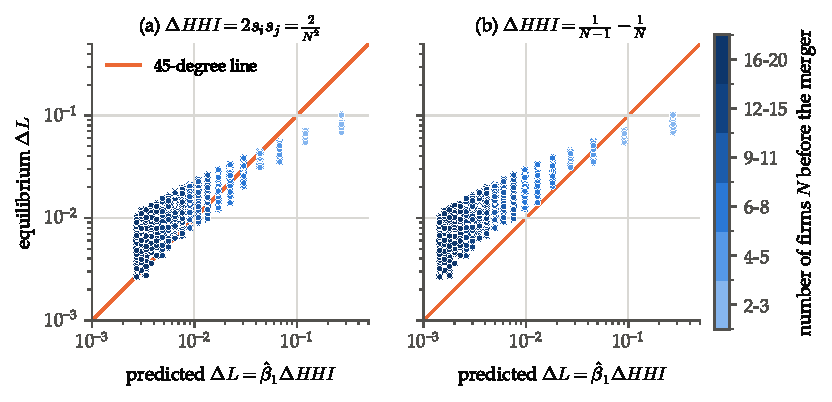
\includegraphics[width=\textwidth]{figures/appC/merger_mc.pdf}
\caption{Equilibrium against predicted changes in the Lerner index after a merger of two firms in 954
simulated Cournot industries, on logarithmic axes. Predictions multiply the cross-industry slope
$\hat\beta_1 = 0.546$ by the share-based change in concentration (panel a) or by the equilibrium change (panel b).
Colours group industries by the number of firms before the merger. Points above the orange line are mergers
whose effect the regression understates.}
\label{fig:C-merger-mc}
\end{figure}

Three findings stand out. First, the regression gets the direction of the error wrong in a systematic way.
For concentrated industries ($N \le 4$) it overstates the effect of a merger by a factor of about two. For
unconcentrated industries ($N \ge 11$) it understates the effect, and with the equilibrium $\Delta\HHI$ the
prediction is less than a third of the truth. The reason is concavity. The OLS slope 0.546 is a
variance-weighted average of chord slopes, and most of the variation in $\HHI$ comes from concentrated
industries, where the Cournot curve is flat. The local slope averages 1.452 across the 1,000 industries, and it
is largest where $\HHI$ is small.

Second, the share-based formula appears to do better than the equilibrium change in concentration. Overall,
its prediction errs by more than 50 percent in 33 percent of industries, against 71 percent for the equilibrium
version. This is an accident of offsetting errors. The share-based formula overstates the change in
concentration by the factor $\frac{2(N - 1)}{N}$, close to two in unconcentrated industries, and this offsets
part of the slope's understatement there. A correct input combined with a wrong slope produces a worse
prediction.

Third, the error comes from the common slope, and the linear approximation does little harm. The local-slope
benchmark misses by more than
50 percent in only 5.5 percent of industries, all of them concentrated. Its remaining error comes from
concavity, since the tangent at the pre-merger point is steeper than the chord to the post-merger point, so it
overpredicts in every industry. The high correlations in Panel B reflect the fact that predicted and actual
effects both fall with $N$. They say little about accuracy, since every prediction uses the same slope for all
industries.

\subsection{Computational notes}\label{sec:C-cournot-computation}

The script \texttt{figures/appC/src/cournot\_merger\_mc.py} implements part (i) in the following steps.
\begin{enumerate}
\item Draw $(a, c, b, \ln F)$ in batches from the stated uniform distributions with a fixed seed. Keep draws with
  $x \ge 2$ until 1,000 industries are accepted, then draw $N$ for each industry.
\item Compute $L = \frac{a - c}{a + Nc}$ and $\HHI = \frac{1}{N}$.
\item Run OLS of $L$ on $(1, \HHI)$. Compute HC1 standard errors as the square roots of the diagonal of
  $\frac{n}{n - 2}(X^\top X)^{-1}\big(\sum_k \hat e_k^2 x_kx_k^\top\big)(X^\top X)^{-1}$ (\cref{app:econometrics}).
\item For industries with $N \ge 2$, compute $\Delta L$ from \eqref{eq:C-merger-dL} and the three predictions,
  then summarize by groups of $N$.
\end{enumerate}

\section{What tax pass-through reveals about conduct}\label{sec:C-passthrough}

The first problem showed that the cross-section of margins and concentration cannot reveal conduct. This problem
turns to a source of variation inside one industry, a shock to cost. Excise taxes are a part of marginal cost that
the econometrician observes without any cost data. \citet{Sumner1981} used this fact to test for monopoly pricing in the US cigarette industry. He found that cigarette
prices rose by more than state excise taxes, and he concluded that the industry was neither competitive nor an
effective cartel. This problem derives what a pass-through rate can and cannot reveal about conduct. It checks the
numbers in Sumner's main table and re-estimates his regression on a reconstructed panel. It then adds clustered
inference with a power calculation, a test of constant pass-through, ad valorem taxes, and a way to recover
marginal cost from two kinds of taxes. \Cref{sec:03-sumner} treats the paper as a case study, and
\cref{sec:02-passthrough} develops the theory of pass-through. Here we work through every step on the data.

\subsection{Statement}\label{sec:C-passthrough-statement}

A homogeneous good has twice differentiable inverse demand $P(Q)$ with $P'(Q) < 0$. The \emph{curvature} of inverse
demand is $\chi \equiv -\frac{QP''(Q)}{P'(Q)}$, and the market elasticity is $\varepsilon = -\frac{P}{QP'(Q)} > 0$.
Sellers pay a specific tax $t$ per unit and have marginal cost $c$, constant unless stated otherwise. Industry
conduct is a constant $\theta \in [0, 1]$, and the equilibrium satisfies the supply relation
\begin{equation}\label{eq:C-supply-tax}
P(Q) + \theta QP'(Q) = c + t .
\end{equation}
Competition is $\theta = 0$, monopoly is $\theta = 1$, and symmetric Cournot with $N$ firms is $\theta = \frac{1}{N}$
(\cref{cor:03-benchmarks}). \emph{Pass-through} is $\rho \equiv \frac{\dd P}{\dd t}$, the change in the equilibrium
price per unit of tax.

The data form a balanced state-year panel reconstructed from the historical volume of \emph{The Tax Burden on
Tobacco} (1983, Table 13). It covers 47 states and the District of Columbia annually from 1954 to 1978, a
total of 1,200 observations. Alaska, Hawaii and New Hampshire are excluded. For state $s$ and year $y$, $p_{sy}$ is
the weighted-average retail price per pack and $t_{sy}$ is the combined state and federal excise tax, both in nominal
cents. Both are recorded on November 1 of each year. Municipal taxes are excluded, and the federal tax is 8 cents per
pack throughout. The national consumer price index $CPI_y$ (CPI-U, 1982--84 average equal to 100) deflates prices to
$P_{sy} = \frac{100\,p_{sy}}{CPI_y}$ and taxes to $T_{sy} = \frac{100\,t_{sy}}{CPI_y}$. \Cref{tab:C-panel-stats}
summarizes the panel.

\begin{table}[htbp]
\centering
\begin{threeparttable}
\caption{The state-year cigarette panel, 1954--1978}
\label{tab:C-panel-stats}
\small
\begin{tabular}{@{}lrrrrrr@{}}
\toprule
Variable & Mean & S.d. & Min & Max & Mean 1954 & Mean 1978 \\
\midrule
Retail price $p_{sy}$ (cents per pack) & 34.04 & 10.51 & 18.20 & 66.50 & 22.45 & 56.55 \\
Excise tax $t_{sy}$ (cents per pack) & 15.73 & 4.66 & 8.00 & 29.00 & 11.10 & 20.63 \\
Real price $P_{sy}$ (1982--84 cents) & 90.67 & 9.65 & 64.32 & 126.67 & 83.47 & 86.74 \\
Real tax $T_{sy}$ (1982--84 cents) & 42.73 & 8.92 & 15.34 & 71.60 & 41.28 & 31.64 \\
Tax share $\frac{t_{sy}}{p_{sy}}$ & 0.467 & 0.060 & 0.229 & 0.584 & 0.492 & 0.361 \\
\bottomrule
\end{tabular}
\begin{tablenotes}\footnotesize
\item Notes: 1,200 state-years (47 states and the District of Columbia). The tax is the state excise tax plus the
federal tax of 8 cents. The CPI-U is 26.9 in 1954 and 65.2 in 1978. The median state tax rises from 3 cents in 1954
to 12 cents in 1978, as \citet[n.~8]{Sumner1981} reports, and the mean tax share is close to his 48.7 and 35.5
percent. Of the 1,152 year-to-year transitions within states, 191 involve a tax change, 6 of them decreases, and the
mean change is 2.39 cents. The real tax falls over the sample, as Sumner notes. Source:
\texttt{figures/appC/src/sumner\_passthrough.py}.
\end{tablenotes}
\end{threeparttable}
\end{table}

\begin{enumerate}[label=(\alph*)]
\item Derive the pass-through rate from \eqref{eq:C-supply-tax}, first with constant marginal cost and then with
  marginal cost $c(Q)$ rising in output. What does $\rho > 1$ imply?
\item Show that one pass-through rate identifies only the composite $\kappa \equiv \theta(\chi - 1)$. Work out the
  linear, log, constant-elasticity and symmetric Cournot cases.
\item Sumner writes the price of firm $j$ as $P_j = \frac{\eta_j}{\eta_j + 1}M_j$, where $\eta_j < 0$ is the
  elasticity of the firm's demand and $M_j = X_j\phi + E_j + t$ its marginal cost. He estimates
  $p_{sy} = X_{sy}\psi + \Theta t_{sy} + U_{sy}$. Derive this aggregate equation and the elasticity implied by
  $\Theta$, and check the elasticities he reports.
\item Estimate $p_{sy} = \mu_s + \tau_y + \rho\,t_{sy} + e_{sy}$ with conventional and state-clustered standard errors.
  Test $\rho = 1$ and assess the power of the test.
\item Re-estimate the regression in real terms. Explain why deflating changes the estimate even though the
  regression contains year effects.
\item Let pass-through vary with the real tax and test whether it does.
\item Describe the set of pairs $(\chi, \theta)$ consistent with the estimate.
\item Derive a bound on $\theta$ from the levels of prices and taxes that does not depend on curvature, and
  evaluate it.
\item Show how changes in the mix of brands affect the pass-through of an average price.
\item Derive the pass-through of an ad valorem tax at rate $\tau$ on the consumer price.
\item What additional data would identify $\theta$?
\end{enumerate}

\subsection{Solution}\label{sec:C-passthrough-solution}

\casehead{Part (a)}
We write equilibrium output as a function $Q(t)$ of the tax and differentiate the supply relation. The general
result allows marginal cost $c(Q)$ to rise with output.

\begin{proposition}[Pass-through of a specific tax]\label{prop:C-passthrough}
Replace $c$ by a differentiable marginal cost $c(Q)$ with $c'(Q) \ge 0$ in \eqref{eq:C-supply-tax}. Suppose the
equilibrium is interior and stable, in the sense that $D \equiv (1 + \theta)P' + \theta QP'' - c' < 0$. Then
\begin{equation}\label{eq:C-rho-general}
\rho = \frac{1}{1 + \theta(1 - \chi) + \frac{c'(Q)}{\lvert P'(Q)\rvert}} ,
\end{equation}
and the denominator is positive. With constant marginal cost,
\begin{equation}\label{eq:C-rho-flat}
\rho = \frac{1}{1 + \theta(1 - \chi)} .
\end{equation}
\end{proposition}

\begin{proof}
This is the first form of \cref{prop:03-passthrough}, with $c$ in place of $MC$ and $D$ in place of $J$. Steps 1 to 3
of the proof of \cref{prop:02-pt-general} derive it by differentiating the supply relation with respect to $t$.
Setting $c' = 0$ gives \eqref{eq:C-rho-flat}.
\end{proof}

\Cref{prop:03-passthrough} also gives the elasticity form of \citet{WeylFabinger2013}. Three consequences follow. First, competition with constant marginal cost
($\theta = 0$, $c' = 0$) gives $\rho = 1$ for every demand curve, because price equals marginal cost. Second,
competition with rising marginal cost gives $\rho = \frac{1}{1 + \frac{c'}{\lvert P'\rvert}} < 1$. Sellers bear part
of the tax, because their marginal cost falls as output contracts. Third, for any conduct a steeper marginal cost
curve lowers $\rho$. Hence $\rho \le 1$ under competition whatever the shapes of demand and cost. An estimate
significantly above one rejects competition without any assumption on curvature, which is the robust half of
Sumner's test.

The denominator of \eqref{eq:C-rho-flat} has a simple reading. Perceived marginal revenue is $P + \theta QP'$, and
its slope relative to the slope of demand is
\begin{equation*}
\frac{(1 + \theta)P' + \theta QP''}{P'} = 1 + \theta(1 - \chi) .
\end{equation*}
A tax raises effective cost by $t$, and output falls until perceived marginal revenue has risen by $t$. The price
rises by more than the tax when perceived marginal revenue is flatter than demand, that is, when $\theta > 0$ and
$\chi > 1$.

\casehead{Part (b)}
With constant marginal cost, \eqref{eq:C-rho-flat} rearranges to
\begin{equation}\label{eq:C-kappa}
\frac{1}{\rho} = 1 + \theta(1 - \chi)
\qquad\Longleftrightarrow\qquad
\kappa \equiv \theta(\chi - 1) = 1 - \frac{1}{\rho} .
\end{equation}
The data enter only through $\rho$, and $\rho$ depends on conduct and curvature only through $\kappa$. Every pair on
the hyperbola $\theta(\chi - 1) = \kappa$ generates the same pass-through. If $\rho > 1$, then $\kappa > 0$, and any
$\theta > 0$ fits the data with curvature $\chi = 1 + \frac{\kappa}{\theta}$. Pass-through alone can therefore reject
competition but never monopoly (\cref{prop:03-passthrough-id}).

Four special cases show how curvature disciplines the reading, and \cref{tab:C-curvature} collects them. For
\emph{linear demand} $P = a - bQ$, $P'' = 0$, so $\chi = 0$ and $\rho = \frac{1}{1 + \theta} \le 1$. For \emph{log
demand} $P = a_0 - b_0\ln Q$ with $b_0 > 0$, the derivatives are $P' = -\frac{b_0}{Q}$ and $P'' = \frac{b_0}{Q^2}$.
Hence
\begin{equation*}
\chi = -\frac{Q\cdot\frac{b_0}{Q^2}}{-\frac{b_0}{Q}} = 1 , \qquad \rho = 1 \text{ for every } \theta .
\end{equation*}
The supply relation becomes $P - \theta b_0 = c + t$, a constant dollar markup. For \emph{constant-elasticity demand}
$P = AQ^{-\frac{1}{\varepsilon}}$,
\begin{equation*}
P' = -\frac{1}{\varepsilon}AQ^{-\frac{1}{\varepsilon} - 1}, \qquad
P'' = \frac{1}{\varepsilon}\Big(1 + \frac{1}{\varepsilon}\Big)AQ^{-\frac{1}{\varepsilon} - 2}, \qquad
\chi = -\frac{QP''}{P'} = 1 + \frac{1}{\varepsilon} .
\end{equation*}
Then $1 + \theta(1 - \chi) = 1 - \frac{\theta}{\varepsilon}$, so that
\begin{equation}\label{eq:C-rho-ce}
\rho = \frac{\varepsilon}{\varepsilon - \theta}, \qquad \kappa = \frac{\theta}{\varepsilon}, \qquad
\theta = \varepsilon\kappa .
\end{equation}
For \emph{symmetric Cournot} with $N$ firms and any demand, $\theta = \frac{1}{N}$ gives
$\rho = \frac{1}{1 + \frac{1 - \chi}{N}} = \frac{N}{N + 1 - \chi}$, and a given $\kappa$ requires $\chi = 1 + N\kappa$.

\begin{table}[htbp]
\centering
\begin{threeparttable}
\caption{Curvature, pass-through and the reading of an estimate above one}
\label{tab:C-curvature}
\small
\begin{tabular}{@{}llccl@{}}
\toprule
Demand and conduct & Inverse demand & $\chi$ & $\rho$ & Reading of $\hat\rho = 1.075$ \\
\midrule
Linear, conduct $\theta$ & $a - bQ$ & 0 & $\frac{1}{1 + \theta}$ & impossible, since $\rho \le 1$ \\
\addlinespace
Log, conduct $\theta$ & $a_0 - b_0\ln Q$ & 1 & 1 & impossible, since $\rho = 1$ \\
\addlinespace
Constant elasticity, conduct $\theta$ & $AQ^{-\frac{1}{\varepsilon}}$ & $1 + \frac{1}{\varepsilon}$ &
  $\frac{\varepsilon}{\varepsilon - \theta}$ & $\theta = 0.069\,\varepsilon$ \\
\addlinespace
Any, symmetric Cournot & $P(Q)$, $\theta = \frac{1}{N}$ & $\chi$ & $\frac{N}{N + 1 - \chi}$ & $\chi = 1 + 0.069N$ \\
\addlinespace
Any, monopoly & $P(Q)$, $\theta = 1$ & $\chi$ & $\frac{1}{2 - \chi}$ & $\chi = 1.069$ \\
\bottomrule
\end{tabular}
\begin{tablenotes}\footnotesize
\item Notes: Constant marginal cost. The last column uses $\hat\kappa = 1 - \frac{1}{\hat\rho} = 0.069$ from
specification M0 in part (d). Linear and constant-elasticity demand belong to the power family
$P = a_0 - b_0Q^{\gamma}$, whose curvature $\chi = 1 - \gamma$ is constant, and log demand is its limit as
$\gamma \to 0$ (\cref{ex:02-pt-examples}).
\end{tablenotes}
\end{threeparttable}
\end{table}

The monopoly row connects to \citet{BulowPfleiderer1983}. A monopolist with constant marginal cost passes through
less than one if and only if direct demand is log-concave (\cref{cor:02-bulow-pfleiderer}). An estimate above one,
read as monopoly, therefore requires log-convex demand at the observed prices. Constant elasticity is one such
demand curve, and it is the one Sumner assumes.

\casehead{Part (c)}
\citet[p.~1011]{Sumner1981} starts from the markup rule of firm $j$,
\begin{equation}\label{eq:C-sumner1}
P_j = \frac{\eta_j}{\eta_j + 1}\,M_j \equiv \Theta_jM_j \qquad \text{(his eq.~1)},
\end{equation}
where $\eta_j < 0$ is the elasticity of the demand curve facing firm $j$ (his sign convention). The marginal cost of
firm $j$ is $M_j$. Under monopoly $\eta_j$ is the market elasticity. Under perfect competition $\eta_j = -\infty$ and
the price-cost ratio $\Theta_j$ equals one. Marginal cost is
\begin{equation}\label{eq:C-sumner2}
M_j = X_j\phi + E_j + t \qquad \text{(his eq.~2)},
\end{equation}
with observed cost factors $X_j$, unobserved factors $E_j$ and the tax $t$, which is common to all firms. Sumner
writes $\beta$, $\epsilon_j$, $R$ and $\theta$ where we write $\phi$, $E_j$, $t$ and $\Theta$, and we rename them to
avoid clashes with the book's notation.

Only state-average prices are observed, so Sumner aggregates (p.~1012). Let $S_j$ be firm $j$'s market share, and
define the share-weighted averages $P = \sum_j S_jP_j$, $M = \sum_j S_jM_j$ and $\Theta = \sum_j S_j\Theta_j$. Writing
each firm's terms as deviations from the averages,
\begin{align*}
P = \sum_j S_j\Theta_jM_j
&= \sum_j S_j\big[\Theta + (\Theta_j - \Theta)\big]\big[M + (M_j - M)\big] \\
&= \Theta M + \Theta\sum_j S_j(M_j - M) + M\sum_j S_j(\Theta_j - \Theta) + \sum_j S_j(\Theta_j - \Theta)(M_j - M) \\
&= \Theta M + \sum_j S_j(\Theta_j - \Theta)(M_j - M) .
\end{align*}
The two middle sums vanish because the shares sum to one and $\Theta$ and $M$ are share-weighted means. The last line
is his eq.~3. The remaining sum is the share-weighted covariance of price-cost ratios and marginal costs. Sumner drops
it under any of three conditions. Elasticities vary little across firms, marginal costs vary little, or the two are
nearly unrelated. He supports the approximation with two facts: retail prices vary little across brands within a
market, and all brands are made in one region with a standard technology. He also writes $\Theta = \frac{\eta}{\eta + 1}$
for the share-weighted elasticity $\eta = \sum_j S_j\eta_j$. This step is exact only when all firms face the same
elasticity, because the map from $\eta_j$ to $\Theta_j$ is nonlinear.

Dropping the covariance and substituting \eqref{eq:C-sumner2} gives $P = \Theta(X\phi + E + t)$. In panel form,
\begin{equation}\label{eq:C-sumner4}
p_{sy} = X_{sy}\psi + \Theta\,t_{sy} + U_{sy}, \qquad \psi = \Theta\phi, \quad U_{sy} = \Theta E_{sy}
\qquad \text{(his eq.~4)} .
\end{equation}
The tax coefficient is the price-cost ratio. Competition implies $\Theta = 1$, and any market power implies
$\Theta > 1$. To recover the firm-level elasticity, we invert $\Theta = \frac{\eta}{\eta + 1}$:
\begin{align*}
\Theta(\eta + 1) &= \eta , \\
\eta(\Theta - 1) &= -\Theta , \\
\eta &= \frac{\Theta}{1 - \Theta} .
\end{align*}
Equivalently, the Lerner index of the firms is $\frac{P - M}{P} = 1 - \frac{1}{\Theta} = -\frac{1}{\eta}$.

\Cref{tab:C-sumner1} reproduces Sumner's Table 1 (p.~1017) and adds the implied quantities. The printed
elasticities equal $\frac{1}{1 - \hat\Theta}$ to the reported precision. Since
$\frac{1}{1 - \Theta} = \frac{\Theta}{1 - \Theta} + 1 = \eta + 1$, each printed value is one unit smaller in absolute
value than the exact inversion. The printed figure inverts the markup over cost, $\frac{P - M}{M} = \Theta - 1 =
-\frac{1}{\eta + 1}$, in place of the Lerner index. The two inversions agree to first order in $\Theta - 1$, and the
gap of 3 to 7 percent leaves Sumner's conclusions unchanged. His conclusion uses the same approximation. With
$\Theta = 1.05$, a 1 percent price increase lowers a firm's sales by 20 percent (p.~1019), where the exact inversion
gives 21 percent.

\begin{table}[htbp]
\centering
\begin{threeparttable}
\caption{Sumner's estimates of the tax coefficient and what they imply}
\label{tab:C-sumner1}
\small
\setlength{\tabcolsep}{4.5pt}
\begin{tabular}{@{}lcccccccc@{}}
\toprule
 & \multicolumn{3}{c}{Sumner (1981), Table 1} & \multicolumn{4}{c}{Implied by $\hat\Theta$} & Replication \\
\cmidrule(lr){2-4}\cmidrule(lr){5-8}\cmidrule(l){9-9}
Row & $\hat\Theta$ & S.e. & $\eta$ printed & $t$ for $\Theta = 1$ & $\frac{1}{1 - \hat\Theta}$ &
  $\frac{\hat\Theta}{1 - \hat\Theta}$ & $1 - \frac{1}{\hat\Theta}$ & $\hat\Theta$ (s.e.) \\
\midrule
(1) Dummies, OLS & 1.074 & 0.013 & $-13.5$ & 5.7 & $-13.5$ & $-14.5$ & 0.069 & 1.075 (0.013) \\
(2) CPI, OLS & 1.029 & 0.011 & $-34.5$ & 2.6 & $-34.5$ & $-35.5$ & 0.028 & 1.029 (0.011) \\
(3) CPI, VC & 1.069 & 0.013 & $-14.5$ & 5.3 & $-14.5$ & $-15.5$ & 0.065 & 1.069 (0.013) \\
\bottomrule
\end{tabular}
\begin{tablenotes}\footnotesize
\item Notes: Dependent variable: retail price per pack in cents, 1,200 state-years. Row (1) includes a dummy for each
year (1978 excluded) and each state (Wyoming excluded). Rows (2) and (3) include the national consumer price index and
no dummies. VC is a variance-components GLS estimator with random state and year effects \citep{FullerBattese1974}.
Sumner reports $R^2$ of about 0.99 with dummies and about 0.95 without. ``$\eta$ printed'' is his implied price
elasticity, with his negative sign. The next four columns are computed from his printed $\hat\Theta$, and
$1 - \frac{1}{\hat\Theta}$ is the implied Lerner index. The replication uses the reconstructed panel with
conventional standard errors, as in the paper, and gives $R^2$ of 0.994 for row (1) and 0.985 for row (2).
\end{tablenotes}
\end{threeparttable}
\end{table}

Sumner reports two further checks. First, he lets the price-cost ratio vary with the price,
$\Theta(P) = \gamma_SP^{1 - \lambda_S}$, where $\gamma_S$ and $\lambda_S$ are his $\gamma$ and $\lambda$ (n.~7). The
markup rule $P = \Theta(P)M$ then gives
\begin{equation*}
P = \gamma_SP^{1 - \lambda_S}M
\qquad\Longrightarrow\qquad
P^{\lambda_S} = \gamma_SM
\qquad\Longrightarrow\qquad
P = (\gamma_SM)^{\frac{1}{\lambda_S}} .
\end{equation*}
Substituting \eqref{eq:C-sumner2} and adding an additive or a multiplicative error gives his eqs.~4$'$ and 4$''$,
which he estimates by nonlinear least squares. The value $\lambda_S = 1$ restores a constant ratio
$\Theta = \gamma_S$. The estimates are $\hat\lambda_S = 0.972$ (0.027) and 0.981 (0.026), with
$\hat\gamma_S = 1.029$ and 1.062 (n.~9). The $t$-statistics for $\lambda_S = 1$ are 1.04 and 0.73, so constancy is
not rejected. Second, the pooled equation estimated year by year gives estimates in the range of Table 1 with no
trend. A squared tax term added to the yearly equations is insignificant in most years.

Sumner reads the results in two steps (pp.~1016--1017). Estimates significantly above one reject atomistic competition. The
implied firm elasticities are 13.5 to 34.5 in absolute value. They are far above estimates of the industry elasticity,
which are ``generally between $-0.3$ and $-0.8$.'' His own estimate is about $-0.40$ (n.~10). A cartel would face the
industry elasticity, so he rejects an effective cartel. He adds that with $\Theta = 1.05$ and prices 5 percent above
marginal cost, market power raises the average price by about 3 cents per pack (p.~1019).

The conduct model of part (b) gives Sumner's ratio a structural meaning. With constant-elasticity demand and flat
cost, the Lerner form of \eqref{eq:C-supply-tax} is $\frac{P - c - t}{P} = \frac{\theta}{\varepsilon}$, so
\begin{equation*}
P = \frac{\varepsilon}{\varepsilon - \theta}(c + t), \qquad
\Theta = \frac{\varepsilon}{\varepsilon - \theta} = \rho, \qquad
\eta = \frac{\Theta}{1 - \Theta} = -\frac{\varepsilon}{\theta} .
\end{equation*}
Sumner's firm elasticity is the market elasticity divided by conduct, and his Lerner index $1 - \frac{1}{\Theta}$
equals $\frac{\theta}{\varepsilon} = \kappa$. Without constant elasticity, $\Theta$ is the pass-through $\rho$ but no
longer the price-cost ratio, and the two must be kept apart.

\casehead{Part (d)}
We call Sumner's row (1) specification M0:
\begin{equation}\label{eq:C-M0}
p_{sy} = \mu_s + \tau_y + \rho\,t_{sy} + e_{sy} .
\end{equation}
The state effects $\mu_s$ absorb stable differences in non-tax costs and demand. The year effects $\tau_y$ absorb
national movements in costs and in the price level. Under \eqref{eq:C-sumner4} they absorb $\Theta X_{sy}\phi$ when
non-tax cost is additive in a state and a year component. Identification requires that tax changes within a state,
relative to other states in the same year, be unrelated to shocks to cost and demand. Formally,
$\E[e_{sy} \mid t_{s1}, \dots, t_{sY}] = 0$ for every state, after conditioning on the fixed effects
(\cref{sec:03-sumner-design}).

By the Frisch-Waugh-Lovell theorem, OLS with both sets of dummies equals the regression of $p_{sy}$ on the
two-way demeaned tax. In a balanced panel the demeaned tax is
\begin{equation*}
\tilde t_{sy} = t_{sy} - \bar t_{s\cdot} - \bar t_{\cdot y} + \bar t_{\cdot\cdot} ,
\end{equation*}
where $\bar t_{s\cdot}$, $\bar t_{\cdot y}$ and $\bar t_{\cdot\cdot}$ are the state means, the year means and the
grand mean. Then
\begin{equation}\label{eq:C-fwl}
\hat\rho = \frac{\sum_{s,y}\tilde t_{sy}p_{sy}}{\sum_{s,y}\tilde t_{sy}^2}, \qquad
\hat\rho - \rho = \frac{\sum_{s,y}\tilde t_{sy}e_{sy}}{\sum_{s,y}\tilde t_{sy}^2} .
\end{equation}
The conventional variance estimator assumes independent errors with a common variance,
\begin{equation*}
\hat V_{\text{conv}} = \frac{s^2}{\sum_{s,y}\tilde t_{sy}^2}, \qquad s^2 = \frac{1}{N - K}\sum_{s,y}\hat e_{sy}^2 ,
\end{equation*}
with $N = 1{,}200$ and $K = 73$ coefficients (the tax, 48 state effects and 24 year effects). The cluster-robust
estimator allows any correlation among the errors of one state:
\begin{equation}\label{eq:C-vcl}
\hat V_{\text{cl}} = \frac{G}{G - 1}\cdot\frac{N - 1}{N - K}\cdot
\frac{\sum_s\big(\sum_y\tilde t_{sy}\hat e_{sy}\big)^2}{\big(\sum_{s,y}\tilde t_{sy}^2\big)^2} ,
\end{equation}
with $G = 48$ clusters. Inference uses the $t$ distribution with $G - 1 = 47$ degrees of freedom, whose 97.5 percent
quantile is 2.012 (\cref{app:econometrics}).

\Cref{tab:C-passthrough} reports the estimates. M0 gives $\hat\rho = 1.0746$ with a conventional standard error of
0.0132, which reproduces Sumner's 1.074 (0.013). The $t$-statistic for $\rho = 1$ is 5.64. The clustered standard
error is 0.0340, 2.57 times the conventional one. The $t$-statistic falls to 2.19, with $p = 0.033$ and a 95 percent
interval of $[1.006, 1.143]$. The rejection of competition survives clustering, but by a much thinner margin. Our
replications of Sumner's rows (2) and (3) give 1.029 (0.011) and 1.069 (0.013), equal to his estimates.

\begin{table}[htbp]
\centering
\begin{threeparttable}
\caption{Pass-through regressions on the reconstructed panel}
\label{tab:C-passthrough}
\small
\begin{tabular}{@{}lcccc@{}}
\toprule
Specification & Estimate & S.e. & 95\% interval & $p$ for $\rho = 1$ \\
\midrule
\multicolumn{5}{@{}l}{\emph{Panel A. Nominal cents}} \\
M0: state and year effects, conventional s.e. & 1.075 & 0.013 & $[1.049,\ 1.101]$ & $<0.001$ \\
M0: state and year effects, clustered s.e. & 1.075 & 0.034 & $[1.006,\ 1.143]$ & 0.033 \\
National CPI, OLS, conventional s.e. & 1.029 & 0.011 & $[1.008,\ 1.050]$ & 0.007 \\
National CPI, variance components & 1.069 & 0.013 & $[1.044,\ 1.093]$ & $<0.001$ \\
\addlinespace
\multicolumn{5}{@{}l}{\emph{Panel B. Real cents, state and year effects, clustered s.e.}} \\
M1 & 1.107 & 0.026 & $[1.055,\ 1.158]$ & $<0.001$ \\
Nominal, CPI-scaled state effects, unweighted & 1.102 & 0.026 & $[1.050,\ 1.155]$ & $<0.001$ \\
\addlinespace
\multicolumn{5}{@{}l}{\emph{Panel C. Pass-through varying with the real tax (M2), clustered s.e.}} \\
$\rho(T)$ at the 10th percentile, $T = 29.9$ & 1.097 & 0.039 & $[1.018,\ 1.176]$ & 0.017 \\
$\rho(T)$ at the median, $T = 43.8$ & 1.106 & 0.025 & $[1.055,\ 1.157]$ & $<0.001$ \\
$\rho(T)$ at the 90th percentile, $T = 53.5$ & 1.113 & 0.034 & $[1.044,\ 1.181]$ & 0.002 \\
$\rho(p_{90}) - \rho(p_{10})$ & 0.016 & 0.053 & $[-0.090,\ 0.122]$ & \\
\addlinespace
\multicolumn{5}{@{}l}{\emph{Panel D. Composite identified by pass-through (clustered M0)}} \\
$\hat\kappa = 1 - \frac{1}{\hat\rho}$ & 0.069 & & $[0.006,\ 0.125]$ & \\
\bottomrule
\end{tabular}
\begin{tablenotes}\footnotesize
\item Notes: 1,200 state-years. Clustered standard errors allow correlation within states (48 clusters), and their
intervals and $p$-values use the $t$ distribution with 47 degrees of freedom. Conventional intervals use $N - K$
degrees of freedom, and the variance-components row uses the normal distribution. In M2 the test of $b_2 = 0$ has
$p = 0.76$. The interval for $\kappa$ maps the endpoints of the clustered interval for $\rho$. The CPI-scaled row
differs from M1 only in its weights (\cref{lem:C-deflate}). Source: \texttt{figures/appC/src/sumner\_passthrough.py}.
\end{tablenotes}
\end{threeparttable}
\end{table}

Clustering matters because both the errors and the regressor are persistent within states. The pooled first-order
autocorrelation of the M0 residuals within states is $r_e = 0.64$, and that of the demeaned tax is $r_x = 0.85$.
Taxes change rarely. Of the 1,152 year-to-year transitions within states, 191 involve a tax change, and only 6 of
those are decreases. A standard approximation shows the size of the problem. Suppose that, within a state, the
errors are AR(1) with coefficient $r_e$ and the sample autocorrelation of $\tilde t$ at lag $k$ is close to $r_x^k$.
Then
\begin{equation*}
\Var\Big(\sum_y\tilde t_{sy}e_{sy}\Big)
= \sigma_e^2\sum_{y,y'}\tilde t_{sy}\tilde t_{sy'}r_e^{\lvert y - y'\rvert}
\approx \sigma_e^2\sum_y\tilde t_{sy}^2\Big(1 + 2\sum_{k \ge 1}r_x^kr_e^k\Big)
= \sigma_e^2\sum_y\tilde t_{sy}^2\cdot\frac{1 + r_xr_e}{1 - r_xr_e} .
\end{equation*}
The conventional formula omits the last factor. Its square root is
$\sqrt{\frac{1 + r_xr_e}{1 - r_xr_e}} = 1.83$, with $r_xr_e = 0.848\times0.638 = 0.541$. The cluster-robust ratio of 2.57 is larger, because
the approximation imposes a common geometric decay that the data need not follow. Both numbers say that Sumner's
standard error is too small by a factor of about two or more \citep{BertrandDufloMullainathan2004}.

The power of the clustered test is modest. A two-sided 5 percent test has 80 percent power against deviations from
one of at least $(t_{0.975, 47} + t_{0.80, 47})\times 0.034 = (2.012 + 0.849)\times0.034 = 0.097$. With the
conventional standard error the threshold would be 0.038. The estimated deviation of 0.075 lies below the clustered
threshold. If the true pass-through were 1.075, a test on a new sample of the same size would reject competition
with probability 0.57. The rejection in our sample is evidence against competition, but a replication could easily
have failed to reject.

\casehead{Part (e)}
Specification M1 replaces nominal by real cents:
\begin{equation}\label{eq:C-M1}
P_{sy} = \mu_s + \tau_y + \rho\,T_{sy} + e_{sy} .
\end{equation}
It gives $\hat\rho = 1.107$ with a clustered standard error of 0.026, a 95 percent interval of $[1.055, 1.158]$
and $p < 0.001$ for $\rho = 1$. The estimate is 0.032 higher than in M0. Year effects absorb any common change in the
price level, so the difference needs an explanation.

\begin{lemma}[Deflating a two-way fixed-effects regression]\label{lem:C-deflate}
OLS estimation of \eqref{eq:C-M1} gives the same $\hat\rho$ as weighted least squares estimation of the nominal
equation
\begin{equation*}
p_{sy} = \mu_s\frac{CPI_y}{100} + \tau'_y + \rho\,t_{sy} + u_{sy}
\end{equation*}
with weights $\big(\frac{100}{CPI_y}\big)^2$, where $\tau'_y$ are unrestricted year effects.
\end{lemma}

\begin{proof}
Multiply \eqref{eq:C-M1} by $\frac{CPI_y}{100}$. Since $P_{sy}\frac{CPI_y}{100} = p_{sy}$ and
$T_{sy}\frac{CPI_y}{100} = t_{sy}$,
\begin{equation*}
p_{sy} = \mu_s\frac{CPI_y}{100} + \tau_y\frac{CPI_y}{100} + \rho\,t_{sy} + e_{sy}\frac{CPI_y}{100} .
\end{equation*}
The second term varies only by year, so it is an unrestricted year effect $\tau'_y$. The error is
$u_{sy} = e_{sy}\frac{CPI_y}{100}$. OLS on \eqref{eq:C-M1} minimizes
$\sum_{s,y}e_{sy}^2 = \sum_{s,y}\big(\frac{100}{CPI_y}\big)^2u_{sy}^2$, which is the weighted least squares
criterion for the nominal equation.
\end{proof}

Deflating therefore changes two things. First, the state effects become proportional to the price level. In nominal
terms the state differences in price net of tax grow with inflation, and this is a state-by-year interaction that
year effects cannot absorb. Second, observations from low-price years receive more weight. The CPI rises from 26.9 to
65.2 over the sample, so a 1954 observation has 5.9 times the weight of a 1978 observation. The script separates the
two channels. OLS on the nominal equation with CPI-scaled state effects and no weights gives 1.102 (0.026), and adding
the weights gives 1.107, identical to M1. Most of the change from 1.075 thus comes from the specification of the state
effects. If non-tax costs and margins in each state are fixed in real terms, M1 is the more natural specification.
Both specifications reject $\rho = 1$ at the 5 percent level.

\casehead{Part (f)}
Specification M2 adds a quadratic in the real tax:
\begin{equation}\label{eq:C-M2}
P_{sy} = \mu_s + \tau_y + b_1(T_{sy} - \bar T) + b_2(T_{sy} - \bar T)^2 + e_{sy} ,
\end{equation}
where $\bar T = 42.73$ is the sample mean of the real tax. Pass-through at tax level $T$ is the derivative
\begin{equation*}
\rho(T) = \frac{\partial P}{\partial T} = b_1 + 2b_2(T - \bar T) .
\end{equation*}
It is linear in $(b_1, b_2)$ with gradient $(1, 2(T - \bar T))$. Its variance is therefore
\begin{equation*}
\Var\big(\hat\rho(T)\big) = V_{11} + 4(T - \bar T)V_{12} + 4(T - \bar T)^2V_{22} ,
\end{equation*}
where $V$ is the clustered covariance matrix of $(\hat b_1, \hat b_2)$. The formula is exact here, and the delta
method gives the same expression (\cref{app:econometrics}).

The estimates are $\hat b_1 = 1.105$ (0.025) and $\hat b_2 = 0.00034$ (0.00112), and the test of $b_2 = 0$ gives
$p = 0.76$. Panel C of \cref{tab:C-passthrough} evaluates $\hat\rho(T)$ at three points of the tax distribution. It
is 1.097 (0.039) at the 10th percentile, 1.106 (0.025) at the median and 1.113 (0.034) at the 90th percentile. The
difference between the 90th and the 10th percentiles is $2\hat b_2(T_{90} - T_{10}) = 0.016$, with standard error
0.053 and 95 percent interval $[-0.090, 0.122]$. \Cref{fig:C-rho-T} plots $\hat\rho(T)$ with its confidence band.

\begin{figure}[htbp]
\centering
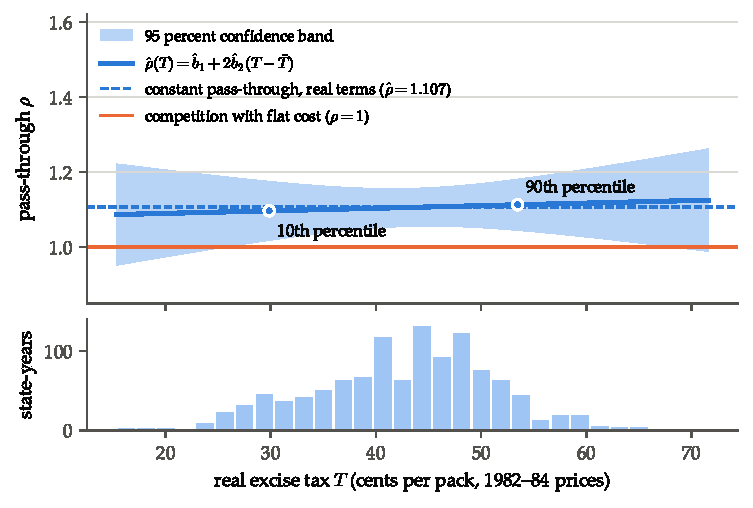
\includegraphics[width=0.86\textwidth]{figures/appC/rho_T.pdf}
\caption{Estimated pass-through as a function of the real excise tax, from specification M2, with a 95 percent
state-clustered confidence band. The dashed line is the constant pass-through of M1, and the orange line is the
competitive benchmark $\rho = 1$. The markers show the 10th and 90th percentiles of the real tax. The lower panel
shows the distribution of the real tax over the 1,200 state-years.}
\label{fig:C-rho-T}
\end{figure}

The data show no sign that pass-through varies with the tax, but the test has little power. With 80 percent power,
a 5 percent test would detect a difference between the two percentiles of $2.861\times0.053 = 0.151$ or more. This
threshold exceeds the estimated excess of pass-through over one in both M0 (0.075) and M1 (0.107). The band in \cref{fig:C-rho-T} also widens at the
extremes, where few state-years lie.

The quadratic also speaks to smuggling. Sumner argues that bootlegging would make the price a concave function of the
tax (n.~6). Bulk sales for shipment out of state lower measured prices in very low-tax states, and illegal
competition lowers them in very high-tax states. Concavity means $b_2 < 0$. Our estimate is positive and
insignificant, in line with his finding that squared tax terms are insignificant in most years.

A flat $\rho(T)$ would be weak evidence for constant-elasticity demand even with a precise estimate. Every member of
the power family in \cref{tab:C-curvature} has constant curvature, so with constant conduct its pass-through is the
same at every tax level. The test asks only whether $\kappa = \theta(\chi - 1)$ is stable over the observed range.
Sumner's estimates of $\lambda_S$ near one make the same point within his family, because $\lambda_S = 1$ makes the
price linear in the tax.

\casehead{Part (g)}
By \eqref{eq:C-kappa}, M0 identifies $\hat\kappa = 1 - \frac{1}{1.0746} = 0.069$. The map from $\rho$ to $\kappa$ is
increasing, so the clustered interval for $\rho$ maps into the interval $[0.006, 0.125]$ for $\kappa$. Every pair
$(\chi, \theta)$ on the hyperbola $\theta(\chi - 1) = 0.069$ fits the estimate equally well, and
\cref{fig:03-identified-set} draws this set with its band. Three points on it illustrate the range.
\begin{itemize}
\item Monopoly ($\theta = 1$) fits with $\chi = 1.069$, a demand curve slightly more convex than log demand.
\item Symmetric Cournot with six firms ($\theta = \frac{1}{6}$) fits with $\chi = 1 + 6\times0.069 = 1.42$.
\item Constant elasticity with an industry elasticity of 0.4 has $\chi = 3.5$. Then \eqref{eq:C-rho-ce} gives
  $\theta = 0.4\times0.069 = 0.028$, with interval $[0.002, 0.050]$. Elasticities of 0.3 and 0.8, the ends of the
  range Sumner quotes, give $\theta = 0.021$ and $0.056$.
\end{itemize}
Under constant elasticity with $\varepsilon = 0.4$, conduct of 0.028 matches symmetric Cournot with about 36 firms.
The industry is close to competitive under that reading. The data alone cannot choose among the three points, and
Sumner's rejection of collusion rests on the constant-elasticity assumption combined with outside estimates of the
elasticity. Even a precise $\hat\theta$ would measure market power only under the static model behind
\eqref{eq:C-supply-tax}. \citet{Corts1999} shows, analytically and by simulation, that the estimated conduct parameter
can badly mismeasure market power when firms sustain tacit collusion in a repeated game (abstract and Section~1). The
estimate need not even be positively correlated with the true elasticity-adjusted margin.

\casehead{Part (h)}
The level of prices and taxes gives a bound that needs no assumption on curvature. With constant marginal cost
$c \ge 0$, divide \eqref{eq:C-supply-tax} by $P$ and use $-\frac{QP'}{P} = \frac{1}{\varepsilon}$:
\begin{equation*}
\frac{P - c - t}{P} = \frac{\theta}{\varepsilon}
\qquad\Longrightarrow\qquad
\theta = \varepsilon\Big(1 - \frac{t}{P} - \frac{c}{P}\Big) \le \varepsilon\Big(1 - \frac{t}{P}\Big) .
\end{equation*}
This is \eqref{eq:03-lerner-bound}. The tax takes a large share of the cigarette price, so the bound is tight. With
$\varepsilon = 0.4$ it gives $\theta \le 0.4\times(1 - 0.467) = 0.213$ at the mean tax share and $\theta \le 0.308$ at
the lowest share in the sample (0.229). If $\theta$ and $\varepsilon$ are the same in every state-year, the highest
share (0.584) gives the tightest bound, $\theta \le 0.166$. Industry elasticities of 0.3 and 0.8 give bounds of 0.160
and 0.426 at the mean share. Every one of these bounds rules out monopoly whatever the curvature. Equivalently,
monopoly at the mean tax share requires an elasticity of at least $\frac{1}{1 - 0.467} = 1.88$ at the observed price,
and at the lowest share at least 1.30.

Under Sumner's constant-elasticity reading, in which $1 - \frac{1}{\rho}$ is the Lerner index (part (c)), the point
estimate also converts into cents. The value $1 - \frac{1}{\hat\rho} = 0.069$ applied to the mean price of 34.0 cents
gives a margin of price over marginal cost plus tax of 2.4 cents per pack. At the 1978 mean price
of 56.6 cents it gives 3.9 cents. Sumner's figure of about 3 cents uses $\Theta = 1.05$, and at the 1978 mean price
this ratio implies a margin of $56.6\times\big(1 - \frac{1}{1.05}\big) = 2.7$ cents.

\casehead{Part (i)}
Sumner's dependent variable is an average over brands. Suppose the measured price is $\bar p = \sum_j w_jp_j$ with
quantity weights $w_j$. Differentiating with respect to the tax,
\begin{equation}\label{eq:C-composition}
\frac{\dd\bar p}{\dd t} = \sum_j w_j\frac{\dd p_j}{\dd t} + \sum_j p_j\frac{\dd w_j}{\dd t} .
\end{equation}
The first term is the average of product-level pass-through, the object that conduct governs. The second is a
composition effect (\cref{rem:02-pt-composition}). A specific tax adds the same amount to every price, which is a
larger percentage of a cheap brand's price. Premium brands become relatively cheaper, consumers trade up, and the
composition term is positive. The regression then overstates product-level pass-through and leans toward rejecting
competition.

A back-of-the-envelope calculation shows how large the composition effect would have to be. Suppose packs come in
an economy and a premium tier whose prices differ by $\Delta$ cents. Suppose also that each price rises one for one
with the tax, as under competition with flat cost. The composition term is then $\Delta\frac{\dd w_H}{\dd t}$, where $w_H$ is
the premium share. Matching $\hat\rho = 1.075$ requires $\frac{\dd w_H}{\dd t} = \frac{0.075}{\Delta}$ per cent of
tax. With a hypothetical gap of $\Delta = 5$ cents, a 10-cent tax increase would have to raise the premium share by
15 percentage points. Two features of the data make shifts of this size unlikely. The Tobacco Tax Council's price
uses fixed national weights for the type of cigarette (regular, king, 100 mm) and the type of sale (carton, single
pack, machine). Shifts across these categories therefore do not move it \citep[p.~1016]{Sumner1981}. Sumner also reports
that retail prices vary little across brands within a market (pp.~1012--1013), so $\Delta$ is small.

A related critique is the quality response of \citet{Barzel1976}. A per-unit tax lowers the relative price of
quality, so higher taxes should raise the quality sold per pack, and with it the price per pack. Sumner replies that
the price data hold the obvious quality dimensions fixed and that centralized manufacturing leaves little room for
quality differences across states (p.~1018). He adds that a Barzel effect would bias the estimate upward, which
strengthens the case against an effective cartel. Barzel notes that an ad valorem tax would not have this effect, and
New Hampshire taxed cigarettes ad valorem until 1975. Sumner finds that New Hampshire's residuals from yearly
regressions are as negative after 1975 as before, which speaks against the quality explanation (n.~11).

\Cref{sec:C-logit-bertrand} computes \eqref{eq:C-composition} in a simulated logit market. There the composition term
is 0.0002 with single-product firms and $-0.0005$ with multi-product firms (\cref{tab:C-logit-tax}). Product-level
pass-through is below one, because logit demand is log-concave in a product's own price
(\cref{prop:C-logit-passthrough}). A logit market cannot produce Sumner's estimate through either term.

\casehead{Part (j)}
An ad valorem tax at rate $\tau$ takes the fraction $\tau$ of the consumer price, and sellers receive $(1 - \tau)P$
per unit. In this part $\tau$ denotes the tax rate. The year effects $\tau_y$ carry a subscript and play no role.

\begin{proposition}[Pass-through of an ad valorem tax]\label{prop:C-adval}
Let sellers receive $(1 - \tau)P$ per unit, with $\tau \in [0, 1)$, and let marginal cost $c$ be constant. Write
$\upsilon \equiv \frac{1}{1 - \tau}$, and let $\rho$ be the specific-tax pass-through \eqref{eq:C-rho-flat} at the same
equilibrium.
\begin{enumerate}[label=(\roman*)]
\item The supply relation is $P + \theta QP' = c\upsilon$, and $\frac{\dd P}{\dd\upsilon} = c\rho$.
\item The elasticity of the price with respect to $\upsilon$ is
  \begin{equation}\label{eq:C-adval-elast}
  \varrho \equiv \frac{\dd\ln P}{\dd\ln\upsilon} = \rho\Big(1 - \frac{\theta}{\varepsilon}\Big) .
  \end{equation}
\item $\varrho = 1$ under competition for every demand curve, and under constant-elasticity demand for every conduct.
  For $\theta > 0$, $\varrho > 1$ if and only if $\chi > 1 + \frac{1}{\varepsilon}$.
\end{enumerate}
\end{proposition}

\begin{proof}
(i) Perceived marginal revenue per unit sold is $(1 - \tau)(P + \theta QP')$. Setting it equal to $c$ and dividing by
$1 - \tau$ gives the supply relation. It has the form of \eqref{eq:C-supply-tax}, with effective marginal cost
$m \equiv c\upsilon$ in place of $c + t$. The derivation in the proof of \cref{prop:02-pt-general} applies to any shift
in effective cost, so $\frac{\dd P}{\dd m} = \rho$. Since $\frac{\dd m}{\dd\upsilon} = c$, the chain rule gives $\frac{\dd P}{\dd\upsilon} = c\rho$.

(ii) Multiplying by $\frac{\upsilon}{P}$ gives $\varrho = \rho\frac{c\upsilon}{P}$. The Lerner form of the supply relation
is $\frac{P - c\upsilon}{P} = \frac{\theta}{\varepsilon}$, so $\frac{c\upsilon}{P} = 1 - \frac{\theta}{\varepsilon}$.

(iii) Under competition $\theta = 0$ and $\rho = 1$, so $\varrho = 1$. Under constant elasticity
$\rho = \frac{\varepsilon}{\varepsilon - \theta}$ by \eqref{eq:C-rho-ce}, and
\begin{equation*}
\varrho = \frac{\varepsilon}{\varepsilon - \theta}\cdot\frac{\varepsilon - \theta}{\varepsilon} = 1 .
\end{equation*}
In general, \eqref{eq:C-rho-flat} gives $\varrho = \frac{1 - \frac{\theta}{\varepsilon}}{1 + \theta(1 - \chi)}$ with a
positive denominator. Hence
\begin{equation*}
\varrho > 1
\iff 1 - \frac{\theta}{\varepsilon} > 1 + \theta(1 - \chi)
\iff \theta(\chi - 1) > \frac{\theta}{\varepsilon}
\iff \chi > 1 + \frac{1}{\varepsilon} ,
\end{equation*}
where the last step divides by $\theta > 0$.
\end{proof}

The proposition reverses the roles of the two taxes. Sumner compares $\rho$ with the competitive benchmark of one.
For an ad valorem tax the natural benchmark is proportional pass-through, $\varrho = 1$. Under constant elasticity that
benchmark holds whatever the conduct, because the price is the fixed multiple $\frac{\varepsilon}{\varepsilon - \theta}$
of effective cost. An ad valorem experiment then carries no information about conduct, while a specific-tax
experiment does. With log demand the situation reverses. A specific tax gives $\rho = 1$ for every $\theta$, while
$\varrho = 1 - \frac{\theta}{\varepsilon}$ reveals the Lerner index. Which tax is informative thus depends on curvature,
which reinforces part (b). For revenue-equivalent small taxes, \cref{rem:02-pt-adval} shows that the ad valorem tax
raises the price less whenever $\theta > 0$.

Sumner's data contain some ad valorem variation. State sales taxes on cigarettes ranged from 0 to 6 percent. Sumner
ignores them, arguing that their effect is small because their ratio to $\lvert\eta\rvert$ is small
\citep[n.~4]{Sumner1981}. The reconstructed panel does not record them.

\casehead{Part (k)}
Five kinds of additional data would move from the composite $\kappa$ to conduct itself.
\begin{enumerate}[label=\arabic*.]
\item \emph{Quantities and a demand rotator.} With quantities, demand can be estimated, and a variable that changes
  the slope of demand at a given price separates conduct from the level and slope of marginal cost
  \citep{Bresnahan1982,Lau1982}. \citet[Section~3.1, pp.~1032--1034]{Bresnahan1989} restates the argument. If the slope
  of inverse demand does not depend on the demand shifters, the term $\theta QP'$ is perfectly collinear with $Q$ in the
  supply relation. Then $\theta$ cannot be separated from the slope of marginal cost. Lau's sufficient condition for
  identification is that the demand shifters cannot be separated from $Q$ in inverse demand, which needs at least two
  shifters (fn.~22 credits both papers). A market-wide cost shifter such as a tax moves the equilibrium along one demand curve and cannot do this
  (\cref{sec:03-identification}).
\item \emph{Demand curvature.} Demand estimated over a wide range of prices gives $\hat\chi$, and then
  $\theta = \frac{\hat\kappa}{\hat\chi - 1}$. The precision of $\hat\theta$ depends on how far $\hat\chi$ is from one.
\item \emph{Brand-level prices.} They remove the composition term of \eqref{eq:C-composition} and measure
  product-level pass-through directly.
\item \emph{Firm-specific cost shifters.} They trace out each firm's residual demand, whose slope measures the firm's
  markup (\cref{sec:03-residual-demand}). Direct measures of marginal cost work as in sugar refining
  (\cref{sec:03-sugar}).
\item \emph{A second kind of tax.} Variation in an ad valorem tax alongside the specific tax reveals marginal cost,
  as the next result shows.
\end{enumerate}

\begin{proposition}[Two taxes reveal marginal cost]\label{prop:C-two-taxes}
Let sellers pay a specific tax $t$ and an ad valorem tax $\tau$ on the consumer price, so that they receive
$(1 - \tau)P - t$ per unit. Let marginal cost $c(Q)$ be differentiable with $c' \ge 0$, let conduct $\theta$ be
constant, and suppose the equilibrium is stable. With $\upsilon = \frac{1}{1 - \tau}$,
\begin{equation}\label{eq:C-two-taxes}
c(Q) + t = \upsilon\,\frac{\partial P}{\partial\upsilon}\Big(\frac{\partial P}{\partial t}\Big)^{-1} .
\end{equation}
The Lerner index $\frac{P - \upsilon(c + t)}{P} = \frac{\theta}{\varepsilon}$ is therefore identified from the two
pass-through rates and the observed $P$, $t$ and $\tau$, whatever the curvature of demand and the slope of marginal
cost.
\end{proposition}

\begin{proof}
Perceived marginal revenue net of the ad valorem tax equals marginal cost plus the specific tax:
$(1 - \tau)(P + \theta QP') = c(Q) + t$. Multiply by $\upsilon$ and move every term to the left. Along the demand
curve, output is a function $Q(P)$ of the price, so the equilibrium price solves
\begin{equation*}
\mathcal{F}(P; t, \upsilon) \equiv P + \theta Q(P)P'\big(Q(P)\big) - \upsilon\big[c\big(Q(P)\big) + t\big] = 0 .
\end{equation*}
Stability makes $\mathcal{F}_P = \frac{D_\tau}{P'}$ positive, where
$D_\tau = (1 + \theta)P' + \theta QP'' - \upsilon c' < 0$. By the implicit function theorem,
\begin{equation*}
\frac{\partial P}{\partial t} = -\frac{\mathcal{F}_t}{\mathcal{F}_P} = \frac{\upsilon}{\mathcal{F}_P} ,
\qquad
\frac{\partial P}{\partial\upsilon} = -\frac{\mathcal{F}_{\upsilon}}{\mathcal{F}_P} = \frac{c(Q) + t}{\mathcal{F}_P} .
\end{equation*}
Dividing the second by the first, $\mathcal{F}_P$ cancels and leaves $\frac{c(Q) + t}{\upsilon}$. Multiplying by $\upsilon$ gives
\eqref{eq:C-two-taxes}. The Lerner form of the supply relation then gives $\frac{\theta}{\varepsilon}$.
\end{proof}

The intuition is that both taxes shift effective marginal cost $\upsilon(c + t)$, but by different amounts. A cent of
specific tax raises it by $\upsilon$ cents, while a unit increase in $\upsilon$ raises it by $c + t$. Both shifts pass
through to the price at the same rate, whatever that rate is, so their ratio reveals the level of $c + t$. The
argument needs both taxes to vary independently, conduct that does not depend on the tax mix, and a correct model of
who remits each tax. With the Lerner index in hand, an outside estimate of $\varepsilon$ gives $\theta$, and, if
marginal cost is flat, $\hat\kappa$ then gives $\chi = 1 + \frac{\hat\kappa}{\theta}$. In Sumner's setting, state sales taxes would supply the
ad valorem variation.

The exercise leaves three lessons. A market-wide cost shifter delivers a test of competition that is robust to the
shapes of demand and cost, although clustering shows it to be fragile here. The same shifter identifies conduct only
jointly with curvature, so Sumner's rejection of collusion rests on outside information about demand. Bounds from
the levels of prices and taxes, or a second kind of tax, say more about market power than the pass-through rate
alone.

\subsection{Computational notes}\label{sec:C-passthrough-computation}

The script \texttt{figures/appC/src/sumner\_passthrough.py} produces every number in this section with numpy and
scipy, in the following steps.
\begin{enumerate}
\item Read the panel, check that it is balanced (48 states by 25 years), and form the real price and tax by dividing by
  $\frac{CPI_y}{100}$.
\item For M0 and M1, regress the price on the tax, 48 state dummies and 24 year dummies. Compute the conventional
  variance and the cluster-robust variance \eqref{eq:C-vcl} from the full regression. By the argument behind
  \eqref{eq:C-fwl}, the tax block of the full sandwich equals the expression in \eqref{eq:C-vcl}.
\item For Sumner's row (2), regress the price on a constant, the tax and the national CPI. For row (3), estimate a
  two-way random-effects model by feasible GLS. Estimate the idiosyncratic variance $\sigma_e^2$ from the two-way
  within regression, and the state and year variances $\sigma_\mu^2$ and $\sigma_\tau^2$ from the regressions of state
  means and year means. Transform every variable as
  $v^*_{sy} = v_{sy} - \lambda_1\bar v_{s\cdot} - \lambda_2\bar v_{\cdot y} + \lambda_3\bar v_{\cdot\cdot}$, with
  $\lambda_1 = 1 - \sqrt{\frac{\sigma_e^2}{\sigma_e^2 + Y\sigma_\mu^2}}$,
  $\lambda_2 = 1 - \sqrt{\frac{\sigma_e^2}{\sigma_e^2 + S\sigma_\tau^2}}$ and
  $\lambda_3 = \lambda_1 + \lambda_2 - 1 + \sqrt{\frac{\sigma_e^2}{\sigma_e^2 + Y\sigma_\mu^2 + S\sigma_\tau^2}}$, then run
  OLS. The estimates are $\hat\sigma_e^2 = 0.74$, $\hat\sigma_\mu^2 = 0.55$ and $\hat\sigma_\tau^2 = 0.47$.
\item For the decomposition of part (e), regress the nominal price on the tax, the state dummies multiplied by
  $\frac{CPI_y}{100}$ and the year dummies, first by OLS and then with weights $\big(\frac{100}{CPI_y}\big)^2$. Check
  that the weighted estimate equals M1 to machine precision.
\item For M2, center the real tax at its mean, add its square, and evaluate $\hat\rho(T)$ and its standard error at
  the 10th, 50th and 90th percentiles of $T_{sy}$.
\item Compute $\hat\kappa$, the points on the identified set, the Lerner bounds, the residual autocorrelations, and
  the power calculations from the stored estimates, and draw \cref{fig:C-rho-T}.
\end{enumerate}
An optional check with \texttt{statsmodels} reproduces the M0 coefficient and both standard errors to $10^{-9}$.
